\chapter{Ligand specificity and dynamics in the \textit{mup} cluster domains}
\label{cha:chap6}

\section{Introduction}
\label{sec:chap6-Intro}
This chapter focusses on understanding two observations made in two different unrelated studies in the \textit{mup} cluster. The first study builds on work conducted in Prof. Thomas' group by Dr. Joanne Hothersall in order to identify the tailoring enzyme responsible for the synthesis of the 6-hydroxyl of mupirocin. According to the position of the 6-hydroxyl (Figure \ref{fig:mupirocin}) in the mupirocin molecule it was hypothesized that the enzyme responsible must be acting after MmpD. Dr. Hothersall proposed MupA may be the likely candidate and therefore in order to confirm her prediction she created two different mutants \textit{$ \Delta $mupA} and \textit{mupA} G127A, D134A. The point mutations were chosen by comparison of MupA with other oxygenases, e.g. PedJ, to identify the active site residues. MupA belongs to the reduced flavin mononucleotide (FMNH$ _{2} $)-dependent oxygenase family of proteins that are responsible for the addition of a hydroxyl group to the substrates in many different metabolic pathways \parencite{El-Sayed2003}. Bioassay and HPLC showed that the deletion strain had no biological activity and wasn't producing pseudomonic acid A; and that the \textit{mupA} G127A, D134A mutant strain was essentially like wild type \textit{Pseudomonas fluorescens} NCIMB 10586. The strains were sent to our collaborators in Bristol for analysis by HPLC, LC-MS and proton NMR, which confirmed these results. They found that the deletion strain produced mupiric acid but not mupirocin H \parencite{Wu2008}. Mupiric acid is thought to be formed by the release of an intermediate from module 4 of MmpD. Since no intermediates longer than mupiric acid were found this fits with the idea that MupA is acting after MmpD. However, it doesn't confirm that it is the 6-hydroxylase. 

This observation raised a new question that, if MupA is responsible for 6-hydroxylation and the deletion strain therefore produces a product with no 6-hydroxyl ($ \alpha $-hydroxyl) and does not progress beyond MmpD, what prohibits the non hydroxylated molecule from proceeding further in the synthesis pathway. It was hypothesized that the KS-mupA2 in the second module of the MmpA subunit might be specific for the $ \alpha $-hydroxylated intermediate and that in the absence of a $ \alpha $-hydroxyl it does not catalyse Claisen condensation. To determine what in the KS-mupA2 might recognise the $ \alpha $-hydroxyl, a docking study was performed in which the modelled KS-mupA2 dimer was docked with the expected cognate mupirocin intermediate. The docking was performed to reproduce the decarboxylation stage of the Claisen condensation with the substrate attached to the catalytic cysteine in the KS active site and the extender molecule (malonate) attached to phosphopantetheine of the ACP, positioned ready for decarboxylation and subsequent elongation of the substrate. The cognate ACP-mupA2 was docked attached to the phosphopantetheine with distance restraints to ensure that the phosphopantetheine was stretched along the active site tunnel. Key residues for hydroxyl recognition as suggested by docking and sequence analysis were investigated by mutagenesis experiments carried out by Miss Yousra Alsamarraie from Prof. Thomas' group. 

The second study discussed here arose from observations during the molecular dynamics simulations of an ACP-mupA3a:MupH complex described in Chapter \ref{cha:chap4}, Section \ref{sec:chap4acpmuphmd}. The 50 ns long simulations of the complex revealed a movement in two loop regions covering the MupH active site. These loop movements suggested that they might be assisting in the accommodation of the ligand upon ACP-mupA3a/b docking to MupH. In order to understand this phenomenon, the variation in distance between the two loops was measured during the ACP-mupA3a:MupH simulations as well as simulations of the, ACP-mupA3a:MupH dimer, MupH wild type monomer and MupH monomer C115 acetylated. The idea behind simulating the ACP-mupA3a:MupH dimer was to see if the dimeric state of MupH (if it exists as a dimer) would affect the loop movements. The MupH monomer acetylated at C115 was simulated to see if the acetylation of the catalytic cysteine in the MupH alone would also trigger the same loop movements. Simulation of the non-acetylated wild type MupH monomer was used as a control.

\section{Results}
\label{chap6:results}
	
	\subsection{A loop at the KS dimer interface appears to be responsible for the substrate specificity}
	\label{sec:ksspecificity}
	In order to understand what might be responsible for KS-mupA2 not to accepting the acyl chain that lacks the $ \alpha $-hydroxyl (6-hydroxyl in the final mupirocin molecule), the expected natural substrate of KS-mupA2 was docked into a homology model of the KS-mupA2 dimer structure (as described in Section \ref{sec:Ks2Docking}). The KS-mupA2 dimer along with the docking domains was modelled using the X-ray structure of the KS-AT dimer from DEBS module 3 (PDB ID 2QO3, \parencite{Tang2007}), as described in Section \ref{sec:KS2modelling}. Docking was performed to reproduce the decarboxylation stage of the Claisen condensation reaction mechanism described in Section \ref{sec:KS}. KS dimer crystal structures show that the active site is made from atoms from both the KS subunits, which was thus also seen in our MupH model and MupH residues within a 5 \AA \ radius of the docked $ \alpha $-hydroxyl included a motif D128, N129, Y130, K131 on the loop of the subunit not covalently carrying the substrate. 
	
	Figure \ref{fig:cartoonAndSurface} shows the overall docked complex with the lowest energy. Figure \ref{fig:closeuploop} shows the closeup view of the loop with the residues within 5 \AA \ radius of the $ \alpha $-hydroxyl highlighted. Figure  \ref{fig:closeuploop} also shows the backbone NH atoms of residues C158 and A403 which were used to restrain the acyl chain close to the catalytic cysteine (C158) in order to mimic the oxyanion hole during acyl chain transfer. Residues F219, H293 and H333 were used to restrain malonate within the active site in order to mimic the decarboxylation step, since these are implicated in decarboxylation as discussed in Section \ref{sec:KS}. The catalytic serine S38 of ACP-mupA2 was restrained to be within 2 \AA \ of the phosphate of the phosphopantetheine. 
	
		\setlength\fboxsep{5pt}
		\setlength\fboxrule{1.5pt}
		\begin{sidewaysfigure}[htbp]
		\centering
		\fbox{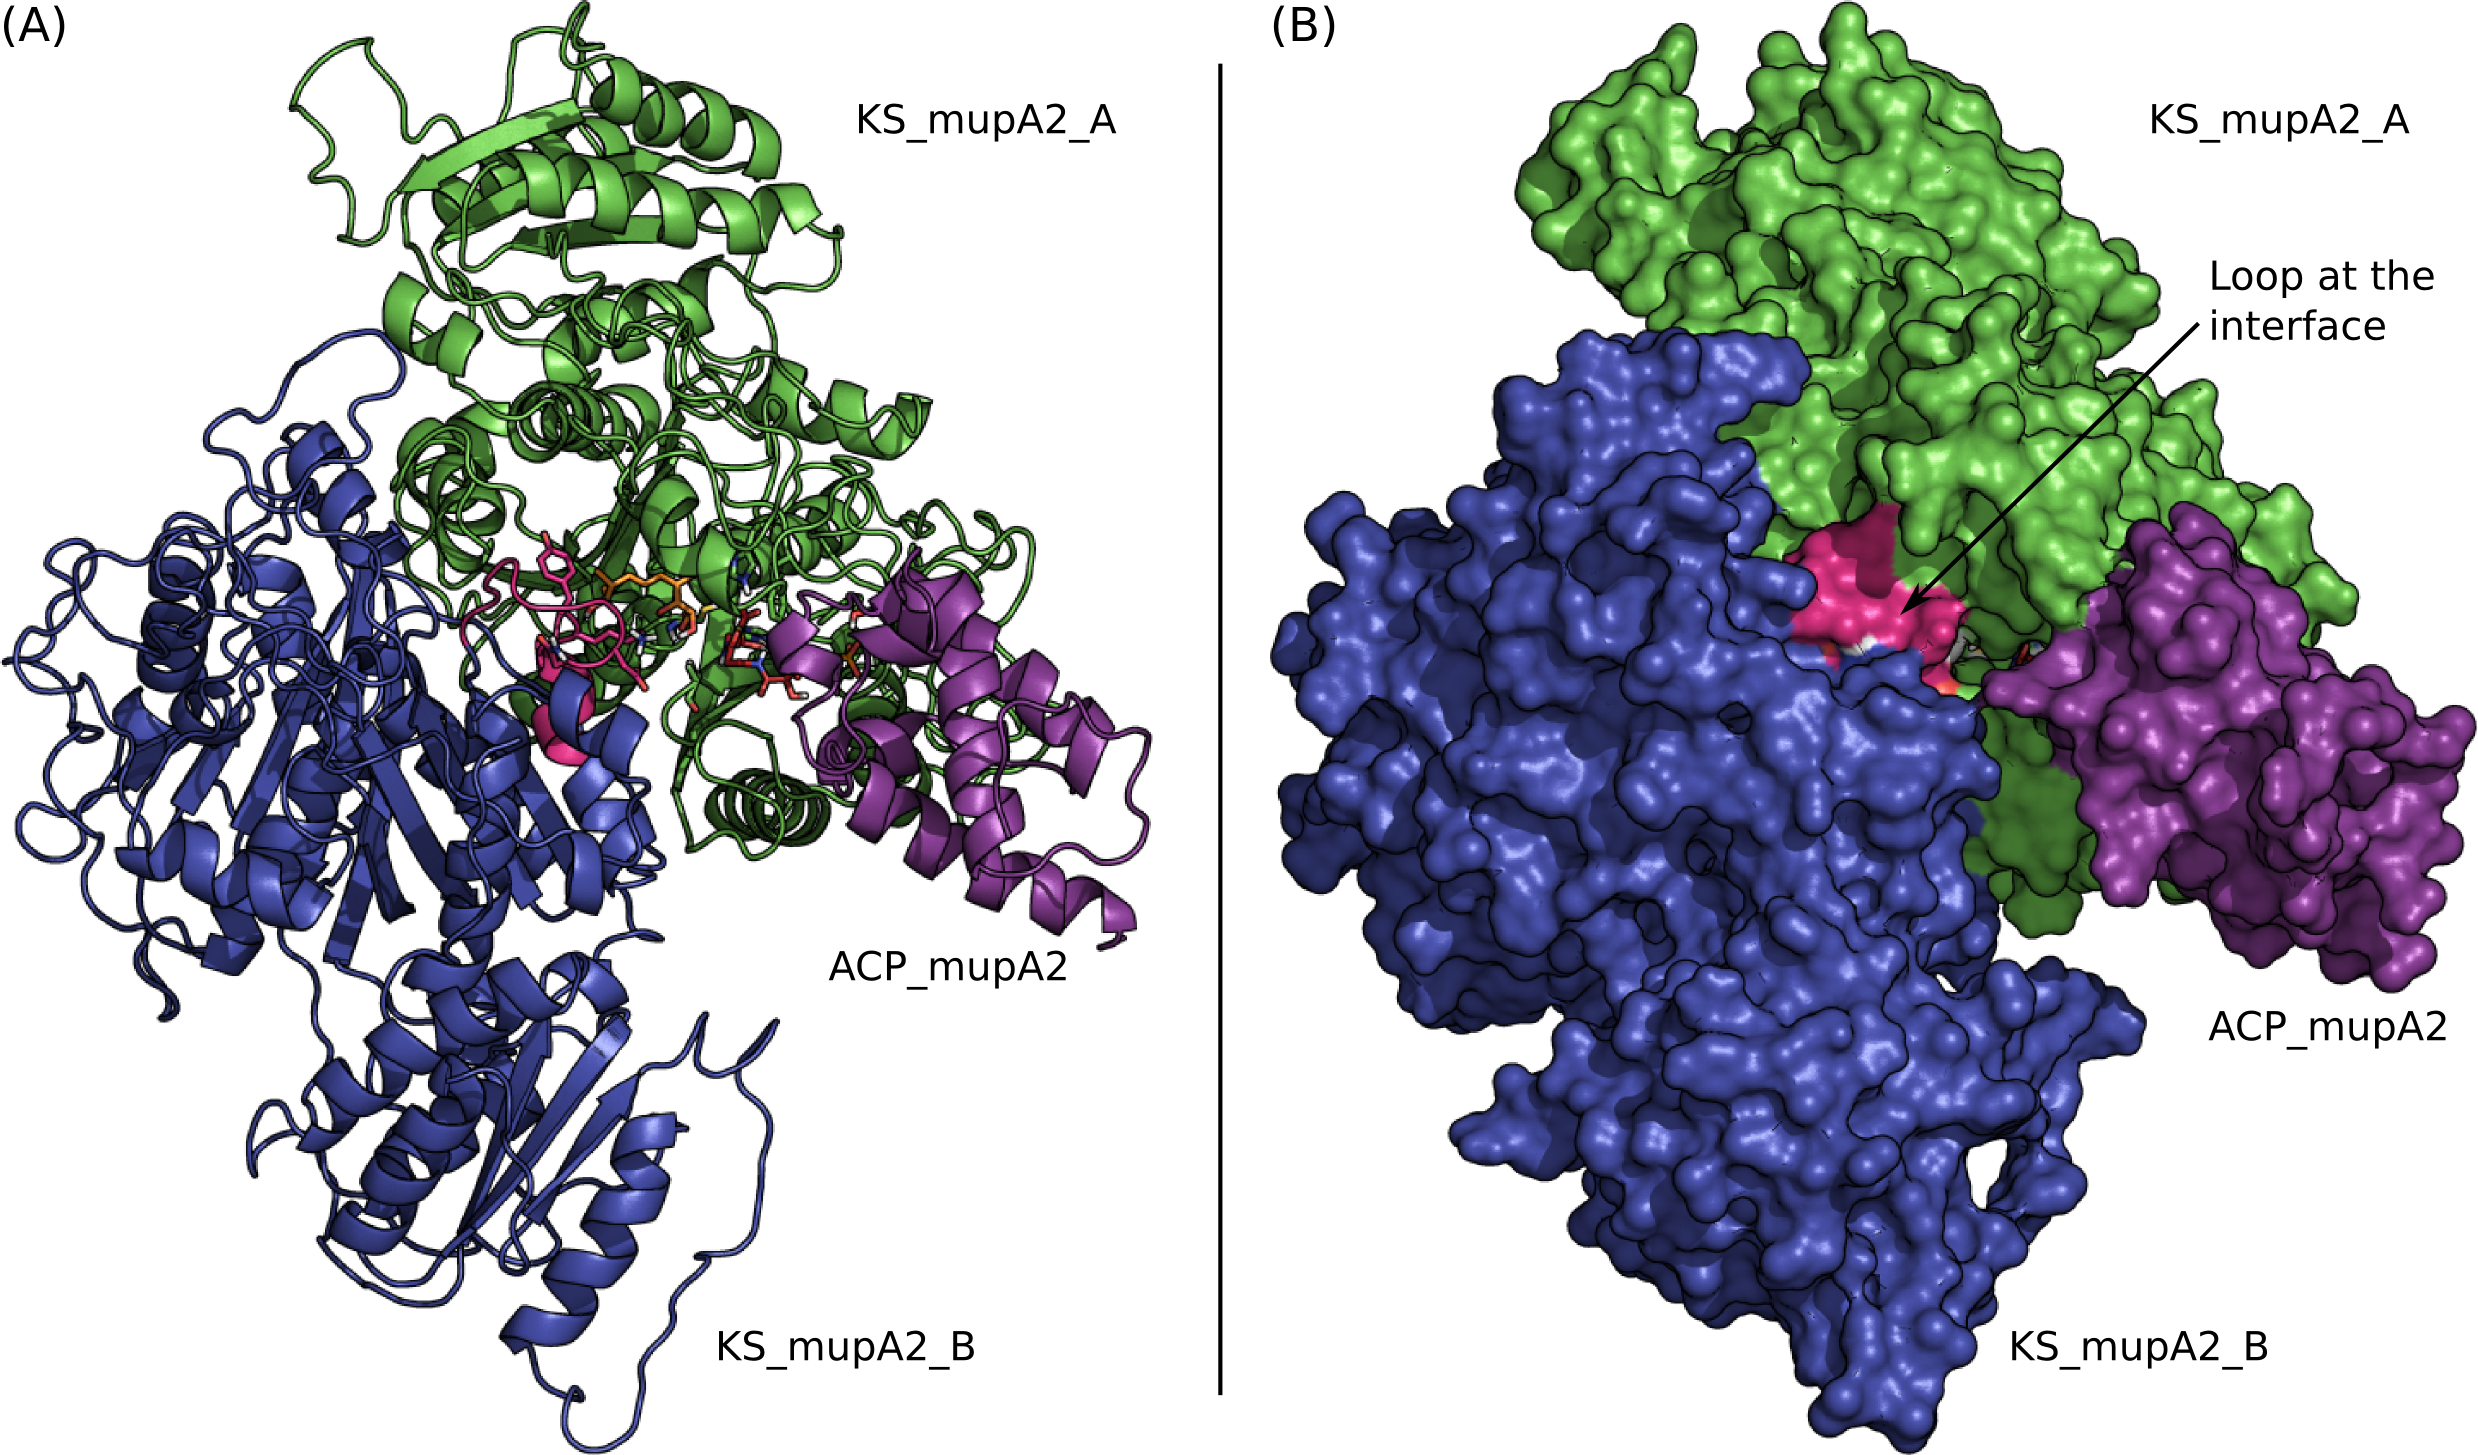
\includegraphics[width=\textwidth,keepaspectratio=true]{graphics/cartoonAndSurface.png}}
		\caption[Cartoon and surface drawings of the KS-mupA2 dimer with ACP-mupA2 docked.]{Cartoon and surface drawings of the KS-mupA2 dimer with ACP-mupA2 docked. Chains A and B of the KS-mupA2 dimer are coloured green and blue respectively with their interface loop coloured pink, ACP-mupA2 is coloured purple. (A) cartoon rendering with phosphopantetheine and polyketide intermediate shown as sticks surrounded by key catalytic residues a zoomed in view of this can be seen in Figure \ref{fig:closeuploop} (B) surface rendering.}
		\label{fig:cartoonAndSurface}
		\end{sidewaysfigure}	

		\setlength\fboxsep{5pt}
		\setlength\fboxrule{1.5pt}
		\begin{figure}[htbp]
		\centering
		\fbox{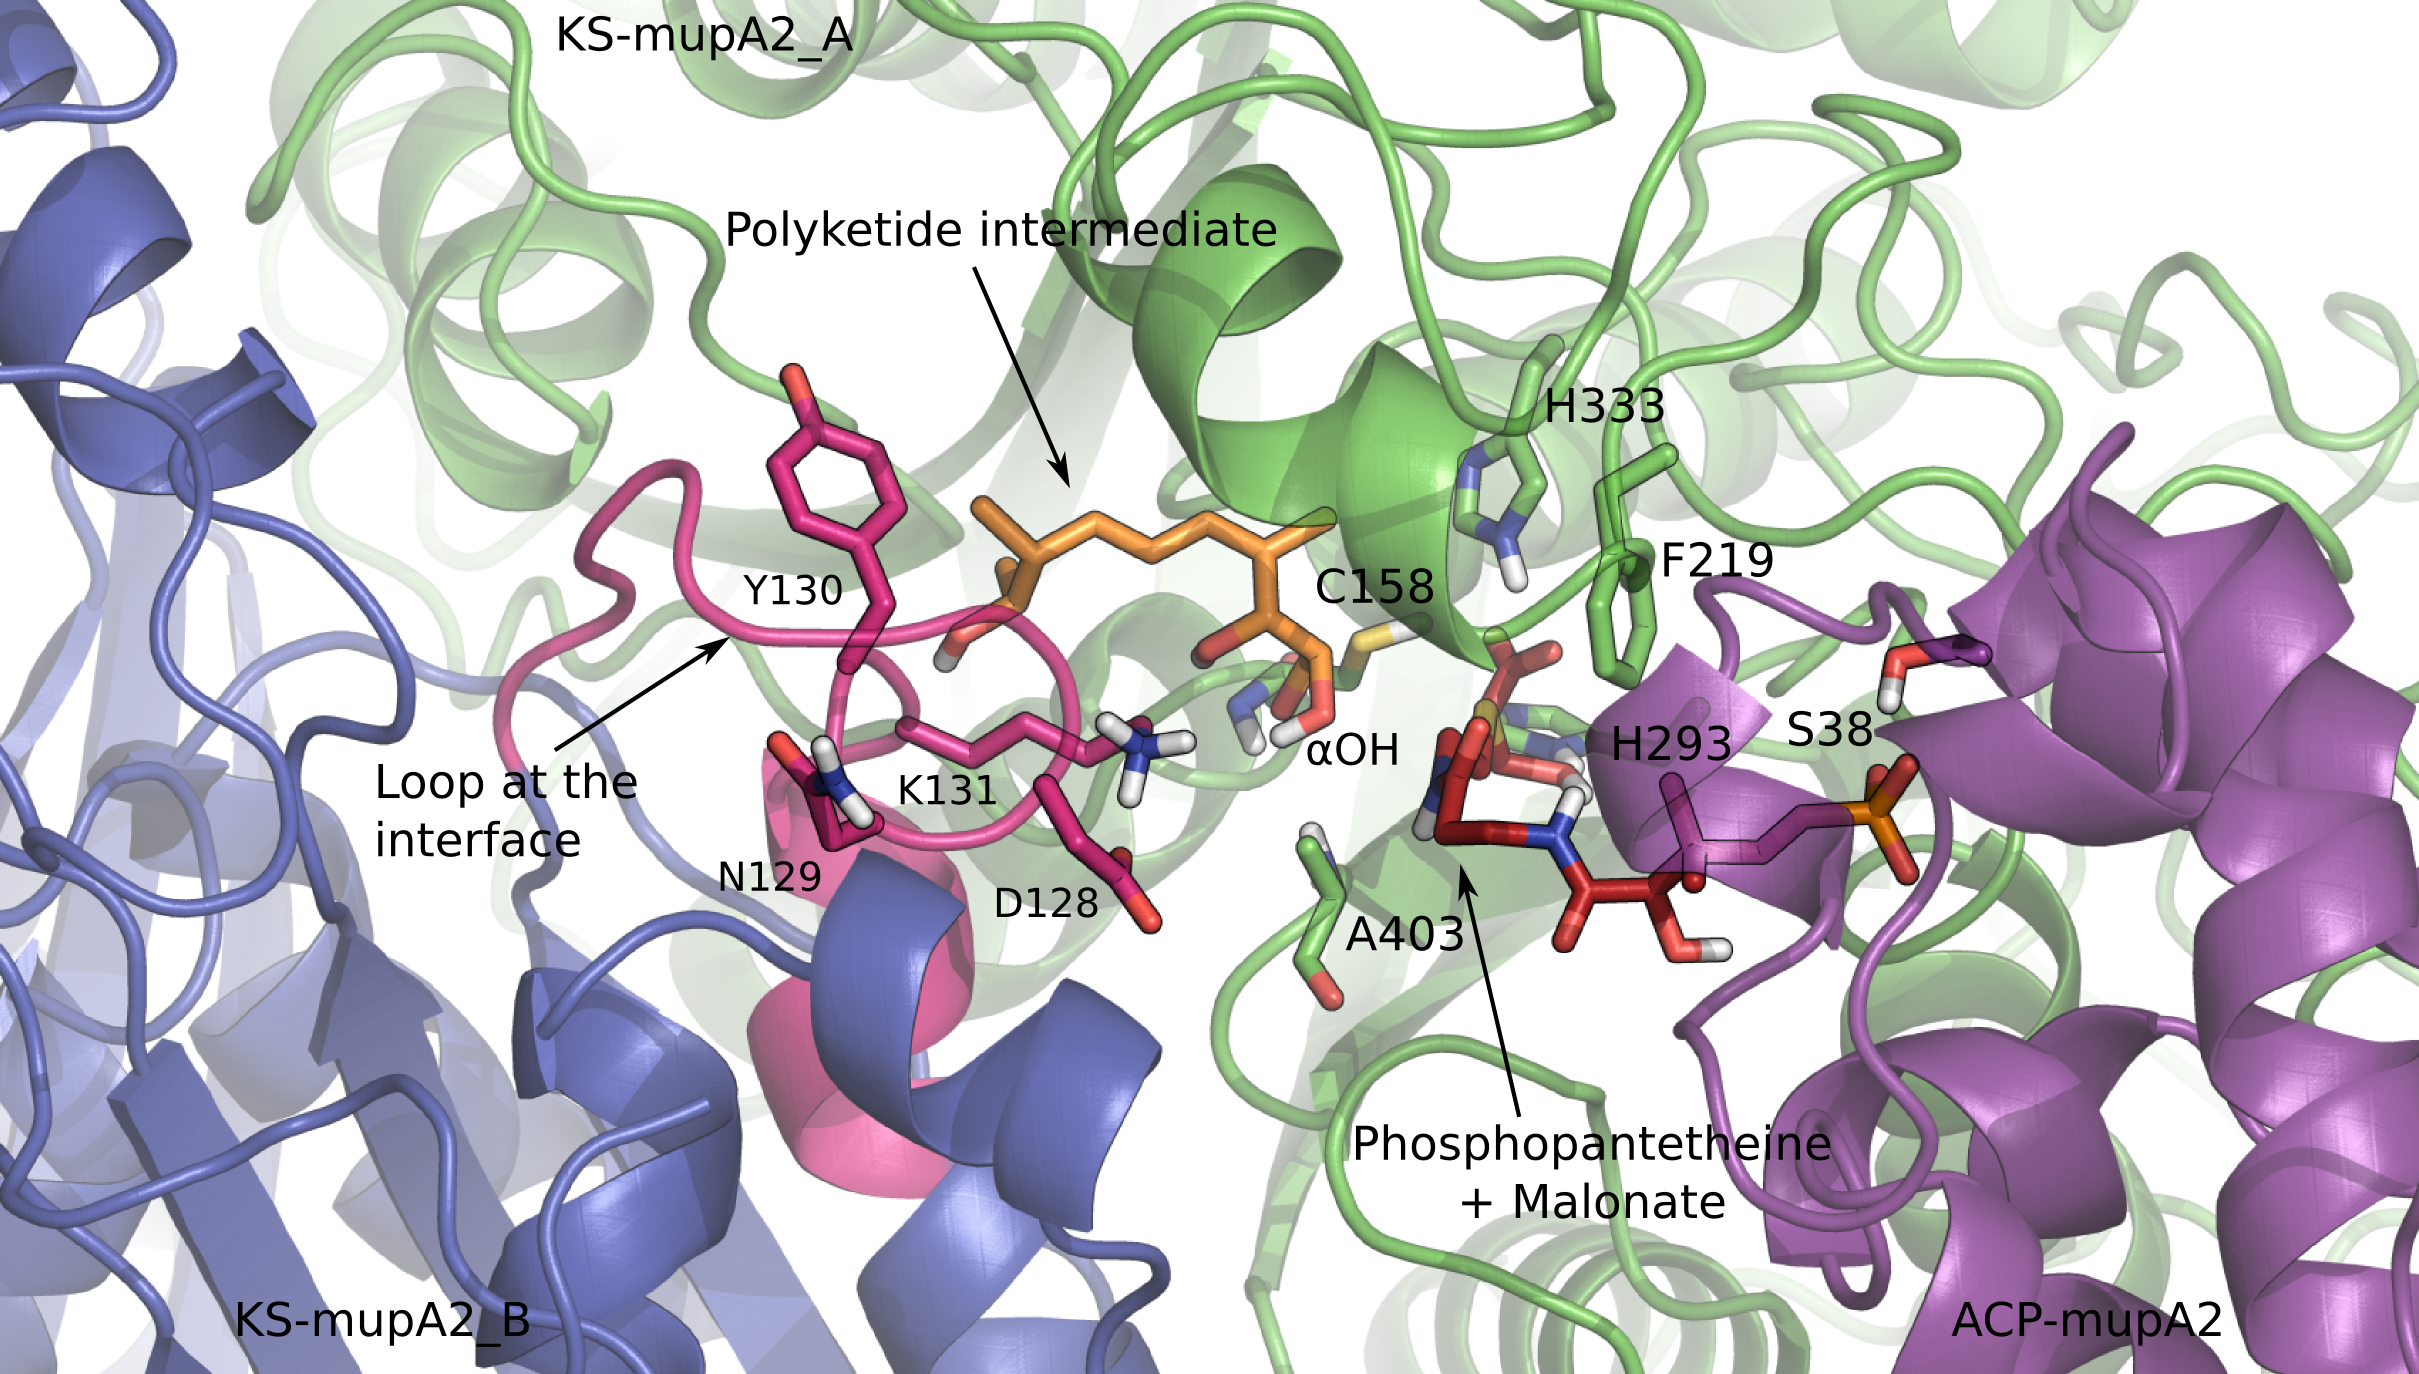
\includegraphics[width=\textwidth,keepaspectratio=true]{graphics/closeuploop.png}}
		\caption[Close up view of the KS-mupA2 dimer and ACP-mupA2 docking interface.]{Close up view of the KS-mupA2 dimer and ACP-mupA2 docking interface. This configuration of substrates represents the decarboxylation/condensation stage of the KS reaction mechanism. Chains A and B of the KS-mupA2 dimer are coloured as green and blue respectively with their interface loop coloured pink, ACP-mupA2 is coloured purple. The DNYK motif is shown as sticks. The malonate extender unit attached to the phosphopantetheine was docked inside the KS-mupA2 active site with three distance restraints requiring it to be 3 \AA \ from each of F219, H293 and H333. The distance between phosphopantetheine and S38 of ACP-mupA2 was restrained to be 2 \AA. The natural substrate of KS-mupA2 was docked inside the active site with three distance restraints of 1.8 \AA \ to the sulphur of C158, and 2.93 \AA \ each to the backbone NH of C185 and A403. The substrate is bound to chain A of the KS whereas the D128NYK motif is predicted to recognise the substrate is on Chain B.}
		\label{fig:closeuploop}
		\end{figure}		
	
	A multiple sequence alignment (Figure \ref{fig:ks_alignment}) of the KS sequences from the mupirocin and thiomarinol clusters revealed that the DNYK motif was conserved in KSs of the second module of MmpA and its equivalent TmpA but not in the other KSs. On the whole much less conservation was found among the other positions in the loop connecting an $ \alpha $-helix at the N-terminus and a \bet-strand at the C-terminus (Figure \ref{fig:ks_alignment}). Based on this observations it was hypothesized that if this loop were swapped with the loops from KS-mupA1 or KS-mupA3, which do not require a substrate with an $ \alpha $-hydroxyl, then the KS mutant might allow the pathway to proceed further. Figure \ref{fig:loopswap} shows the loop region of interest on the KS-mupA2 and the sections of KS-mupA1 and KS-mupA3 to replace it. Miss Yousra Alsamarraie carried out suicide mutagenesis to swap the loops and HPLC to detect antibiotic production.   

		\setlength\fboxsep{5pt}
		\setlength\fboxrule{1.5pt}
		\begin{figure}[htbp]
		\centering
		\fbox{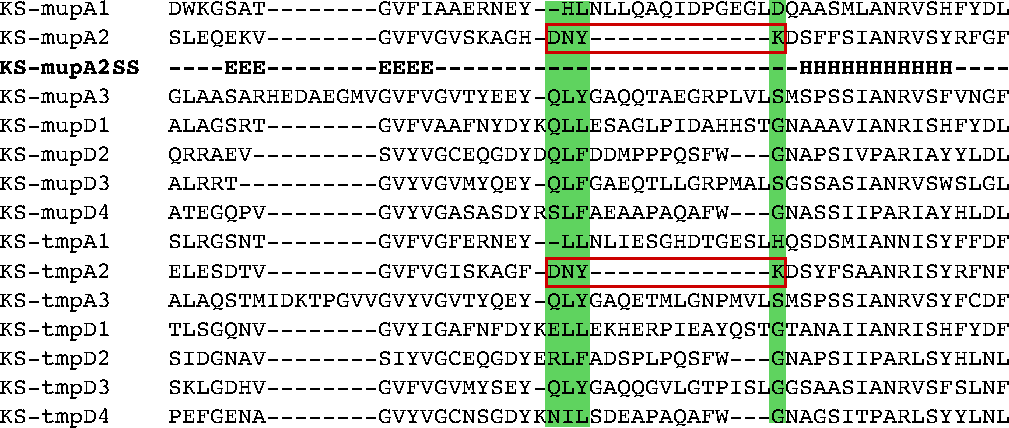
\includegraphics[width=\textwidth,keepaspectratio=true]{graphics/ks_alignment.pdf}}
		\caption[Portion of the multiple sequence alignment of the KS domains from mupirocin (MmpA/D) and thiomarinol (TmpA/D) clusters. ]{Portion of the multiple sequence alignment of the KS domains from mupirocin (MmpA/D) and thiomarinol (TmpA/D) clusters.}
		\label{fig:ks_alignment}
		\end{figure}	

		\setlength\fboxsep{5pt}
		\setlength\fboxrule{1.5pt}
		\begin{figure}[htbp]
		\centering
		\fbox{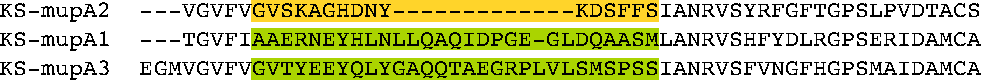
\includegraphics[width=\textwidth,keepaspectratio=true]{graphics/loopswap.pdf}}
		\caption[Region of the loop on the KS-mupA2 which was proposed to be swapped by the loops from KS-mupA1 and KS-mupA3. ]{Region of the loop on the KS-mupA2 which was proposed to be swapped by the loops from KS-mupA1 and KS-mupA3.}
		\label{fig:loopswap}
		\end{figure}	
%		
		At the time of writing this thesis Miss Y. Alsamrarraie was able to replace the loop from KS-mupA2 with the loop of KS-mupA1 in \textit{P. fluorescens} NCIMB 10586 wild type and \textit{P. fluorescens} $\Delta$\textit{mupA} strains. The blue line in Figures \ref{fig:ks1DeltaMupa} and \ref{fig:ks1WildType} show the HPLC trace for the \textit{P. fluorescens} $\Delta$\textit{mupA} strain which was used as the control, there is no peak at 21 mins, which would correspond to pseudomonic acid A production. The red line in Figure \ref{fig:ks1DeltaMupa} shows the HPLC trace for the KS-mupA2 loop replaced with the loop from KS-mupA1 expressed in the \textit{P. fluorescens} $\Delta$\textit{mupA} strain. The trace shows a small peak at around 22:30 mins, which suggests that the substrate was processed by KS-mupA2 however, the metabolite produced still needs to be characterised. The red line in Figure \ref{fig:ks1WildType} shows the HPLC trace for the KS-mupA2 loop replaced with the loop from KS-mupA1 expressed in \textit{P. fluorescens} NCIMB 10586 wild type strain. This trace also shows a small peak at around 22 mins, suggesting that the KS-mupA1 loop is tolerant to both the substrates with and without $ \alpha $-hydroxyl. These samples have been sent to our collaborators in Bristol for LC-MS analysis to determine the structures of the metabolite produced. 

		\setlength\fboxsep{5pt}
		\setlength\fboxrule{1.5pt}
		\begin{figure}[htbp]
		\centering
		\fbox{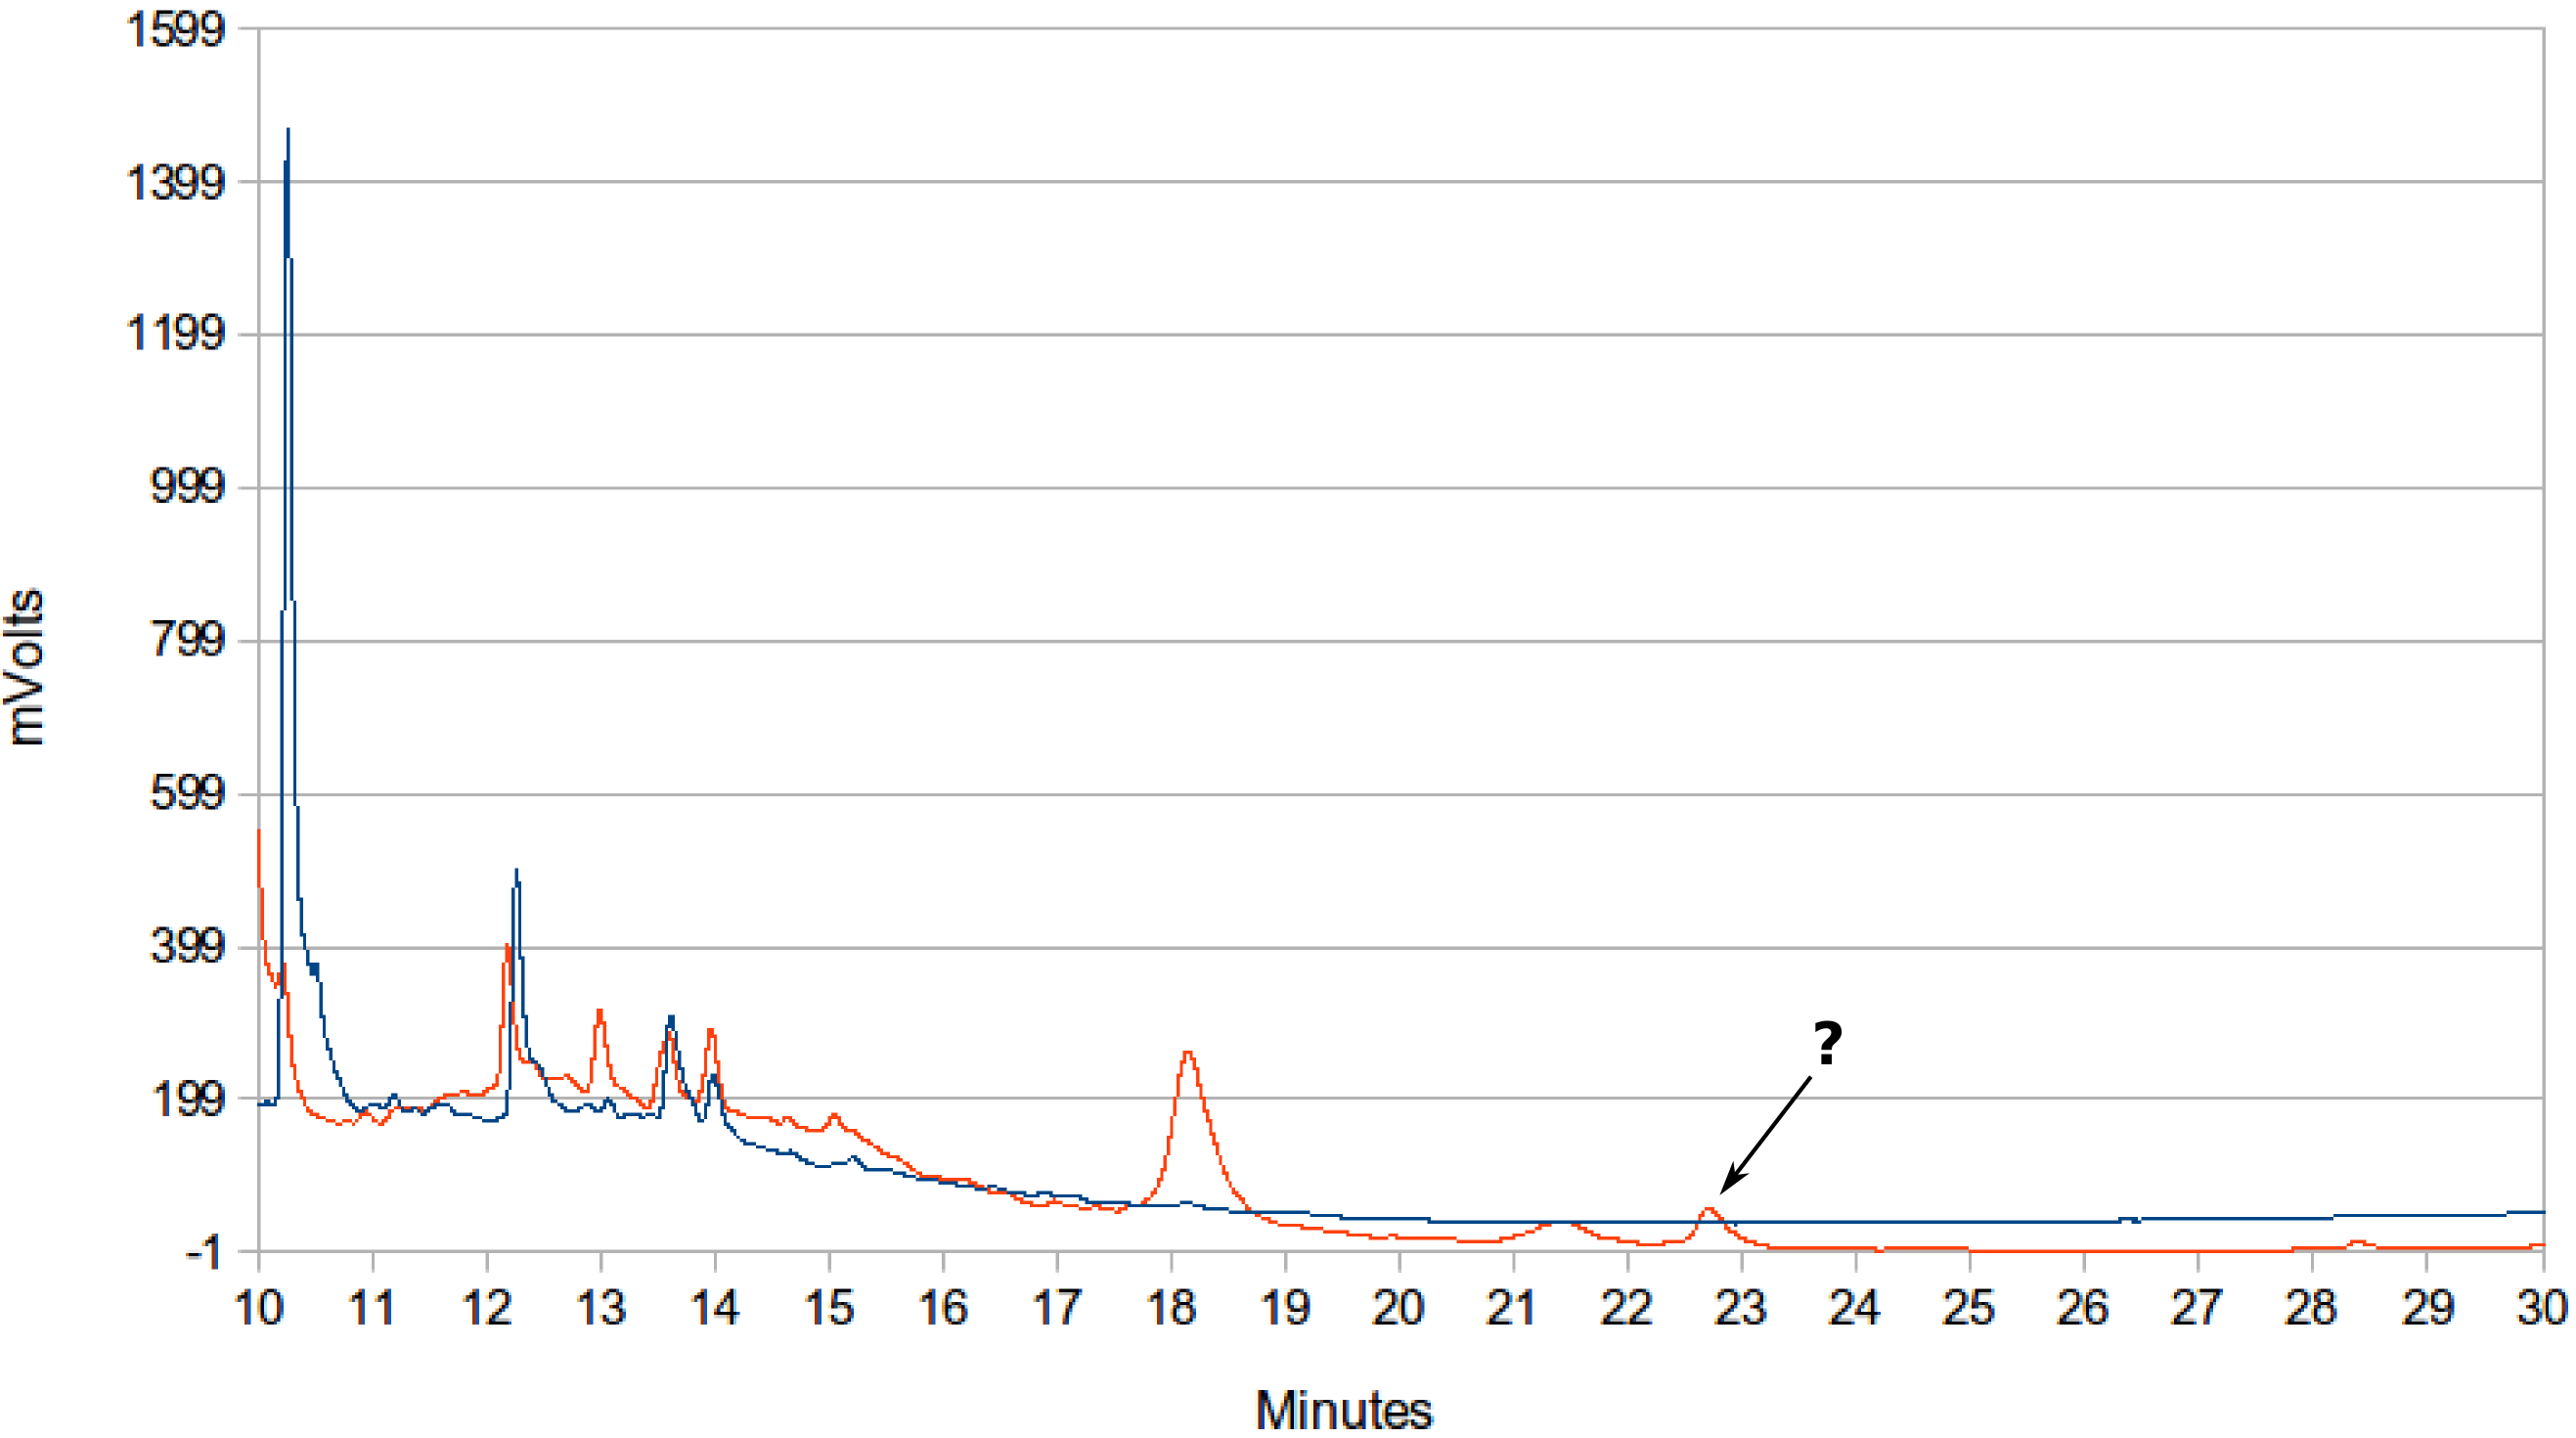
\includegraphics[width=0.9\textwidth,keepaspectratio=true]{graphics/ks1DeltaMupa_new.png}}
		\caption[HPLC trace for the KS-mupA2 loop replaced with the loop from KS-mupA1 in \textit{P. fluorescens} $ \Delta $\textit{mupA} strain.]{HPLC trace for the KS-mupA2 loop replaced with the loop from KS-mupA1 in \textit{P. fluorescens} $ \Delta $\textit{mupA} strain, shown in red. The blue line represents the HPLC trace for \textit{P. fluorescens} $ \Delta $\textit{mupA} strain used as control.}
		\label{fig:ks1DeltaMupa}
		\end{figure}						

		\setlength\fboxsep{5pt}
		\setlength\fboxrule{1.5pt}
		\begin{figure}[htbp]
		\centering
		\fbox{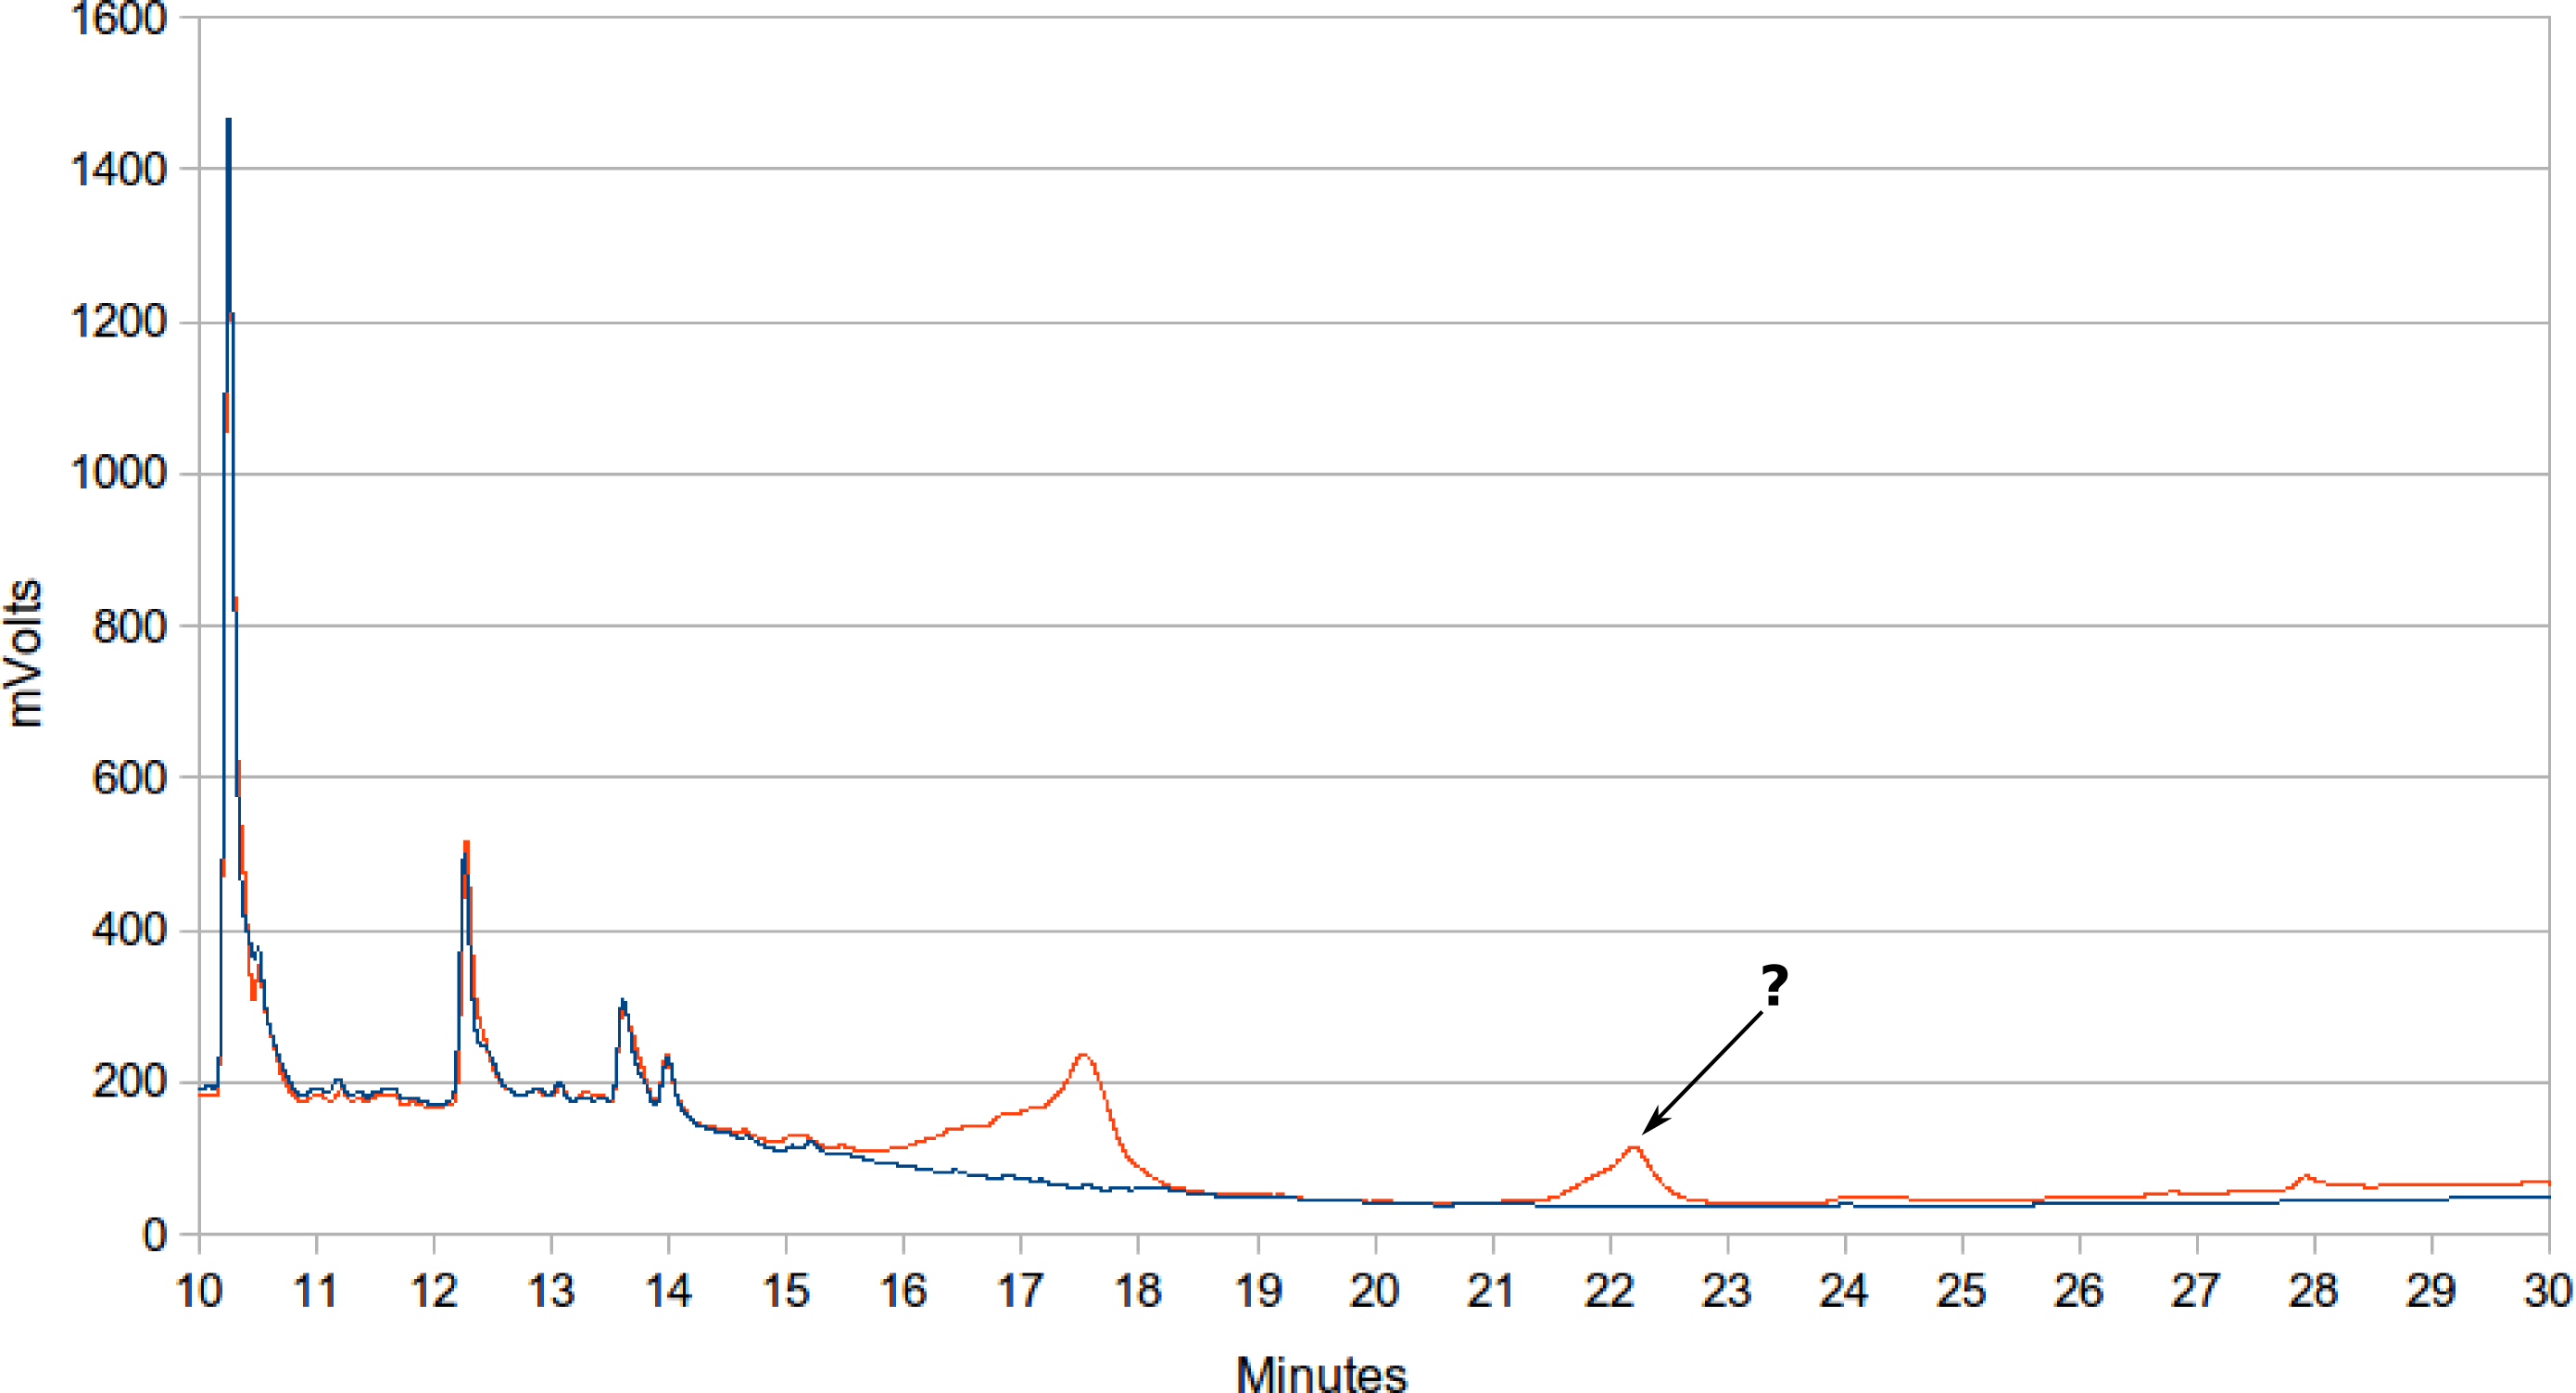
\includegraphics[width=0.9\textwidth,keepaspectratio=true]{graphics/ks1WildType.png}}
		\caption[HPLC trace for the KS-mupA2 loop replaced with the loop from KS-mupA1 in \textit{P. fluorescens} NCIMB 10586 wild type strain.]{HPLC trace for the KS-mupA2 loop replaced with the loop from KS-mupA1 in \textit{P. fluorescens} NCIMB 10586 wild type strain, shown in red. The blue line represents the HPLC trace for \textit{P. fluorescens} $ \Delta $\textit{mupA} strain used as control. }
		\label{fig:ks1WildType}
		\end{figure}				

\newpage		
	\subsection{Movement of MupH surface loops may have a role in ligand binding}
	\label{sec:loopMovement}
	Three independent molecular dynamics simulations of the ACP-mupA3a:MupH complex with the bound substrate, each of 50 ns length, revealed large movements in two loop regions causing a separation between the loops which would otherwise cover the MupH active site tunnel, loop I and II in Figure \ref{fig:muphAligned}. To further explore this observation, each of the three simulations were extended to 100 ns, as described in Section \ref{sec:mdAcpMuph}. Out of the two loops, loop II showed greater movement (Figure \ref{fig:acpMuphMonomerRmsf}) and upon visualizing the movie for the simulation of the ACP-mupA2a:MupH complex the loop movement appears to aid the accommodation of the ligand in the active site by widening the active site tunnel (Figure \ref{fig:muphAligned}). This observation also lead to the hypothesis that such a loop movement in MupH may be required to let a large ligand, like monic acid attached to a phosphopantetheine, to enter inside its active site. Plotting the average of the distances between P207 in loop II and each of L150, M151 and I152 in loop I, for simulation replicate 1 (Figure \ref{fig:AcpSpmMuphCyaSim0}), as well as the average distances between D208 and S209 in loop II and L150, M151 and I152 in loop I %Measuring the distance between the C$ \alpha $ of three residues on loop I and II each replicate 1 
	revealed that the loops widen up to 3 nm during the first 30 ns and then narrow down to around 1 nm the remaining 70 ns. Replicate 2 did not show any huge fluctuation in the distance and replicate 3 showed only moderate fluctuation on two different occasions along the trajectory (Figure \ref{fig:AcpSpmMuphCyaSim1} and \ref{fig:AcpSpmMuphCyaSim2}). The procedure to measure the distances between the loops is described in the methods Section \ref{sec:distLoops}. Table \ref{tab:mupHSimulationSetupSummary} summarizes the different simulations setup for the analysis of loop movements in MupH.

	
	
		\setlength\fboxsep{5pt}
		\setlength\fboxrule{1.5pt}
		\begin{figure}[htbp]
		\centering
		\fbox{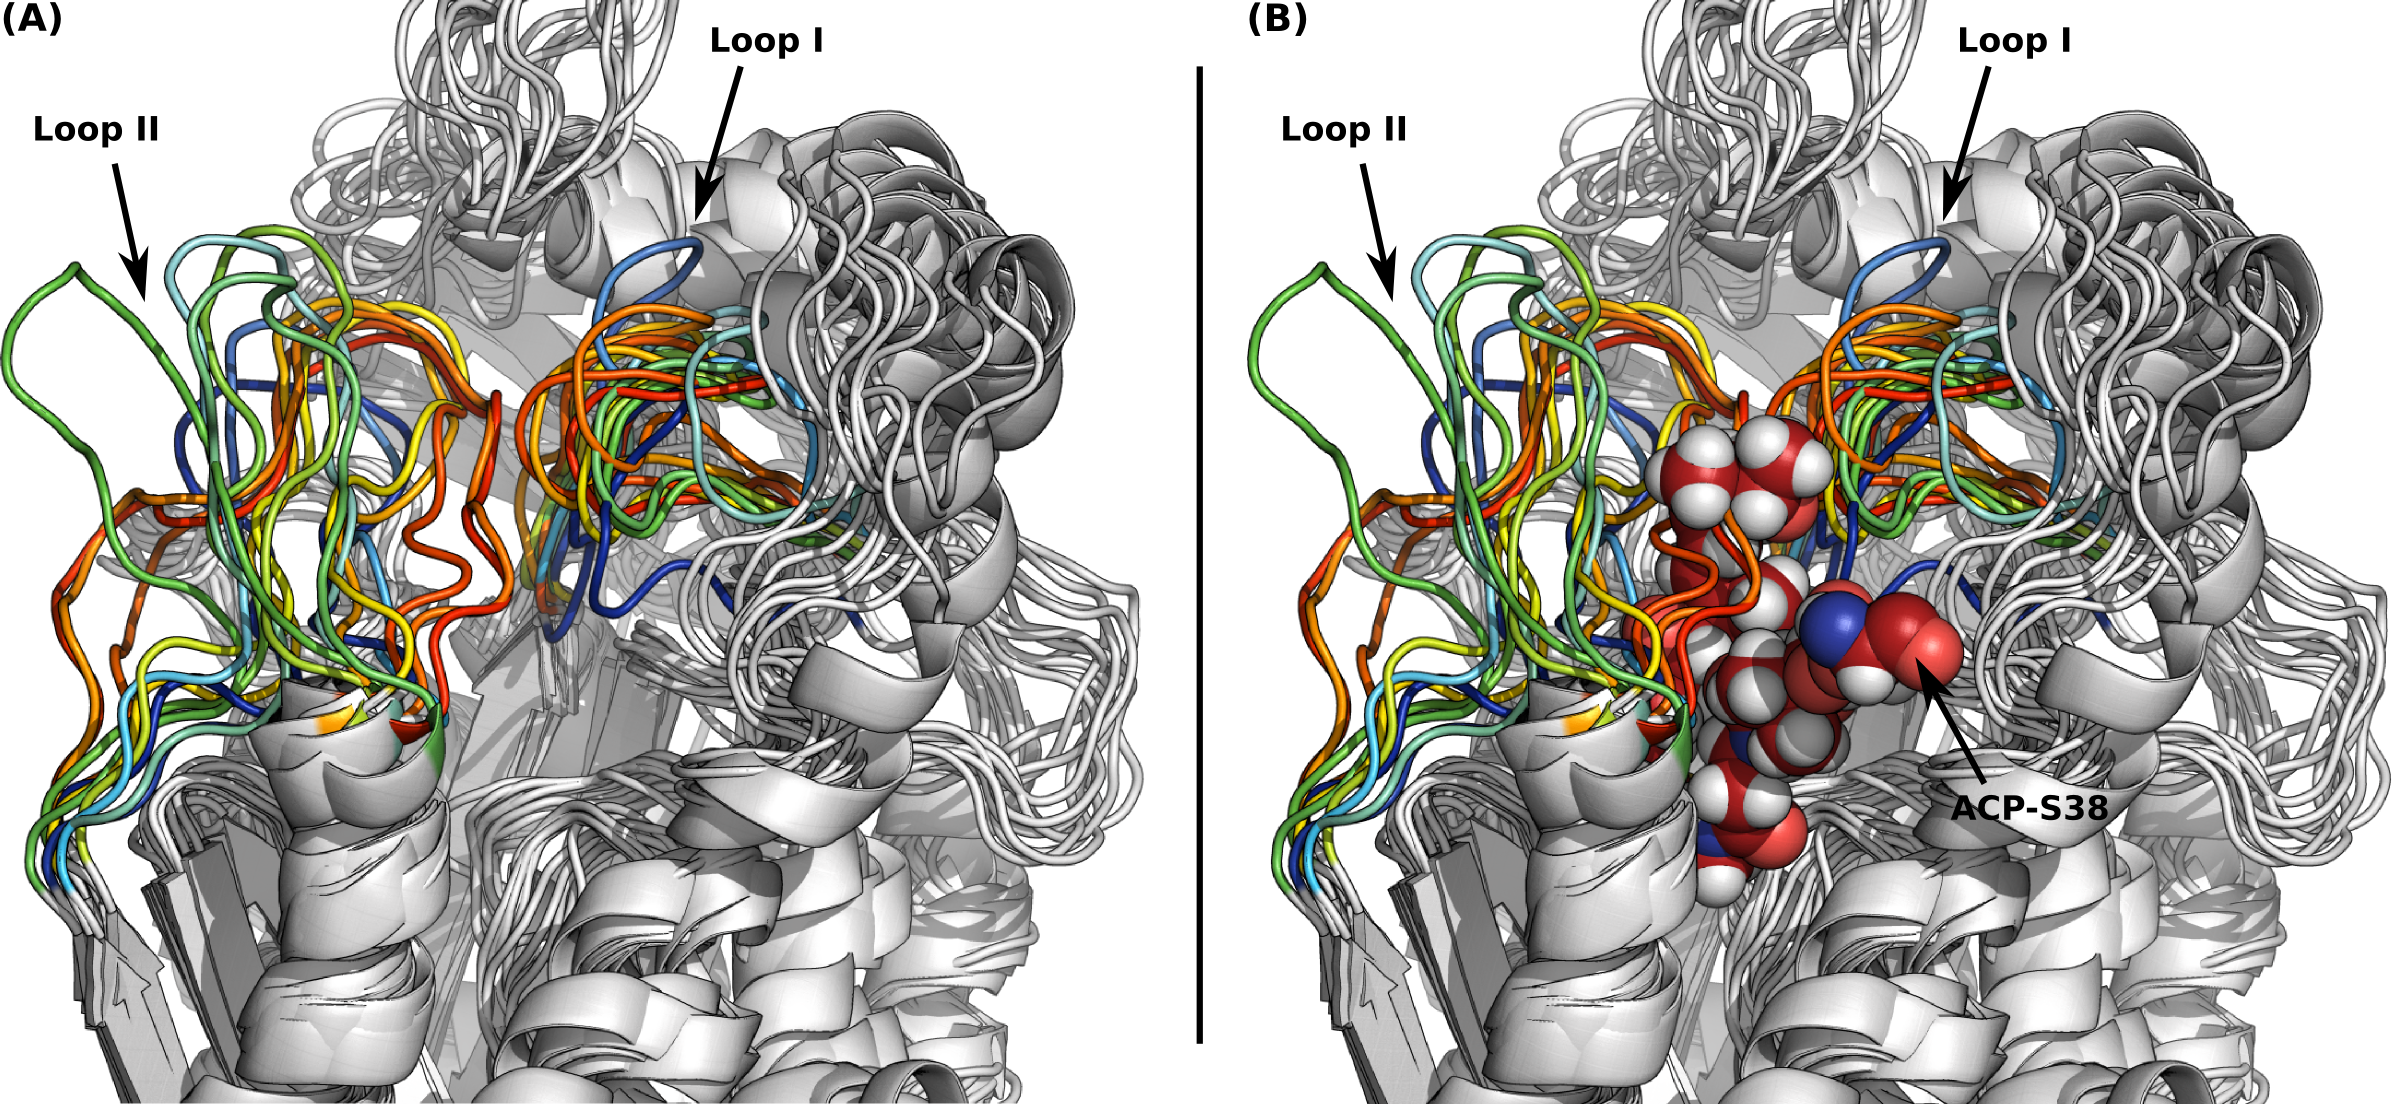
\includegraphics[width=\textwidth,keepaspectratio=true]{graphics/muphAligned.png}}
		\caption[Simulation of ACP-mupA3a:MupH monomer with substrate shows movements of loops over the MupH active site.]{Simulation of ACP-mupA3a:MupH monomer with substrate shows movements of loops over the MupH active site. (A) without and (B) with cognate substrate of MupH attached to the side chain of ACP-mupA3a S38 rendered as spheres. Snapshots at every 5 ns of the 50 ns molecular dynamics simulation revealed the movement in the loop I (residue 147-171) and II (residue 198-214) which may assist in the binding of the ligand. Loop II showed greater movement than loop I. Different coloured loops represent different snapshots. }
		\label{fig:muphAligned}
		\end{figure}	
		
		\setlength\fboxsep{5pt}
		\setlength\fboxrule{1.5pt}
		\begin{figure}[htbp]
		\centering
		\fbox{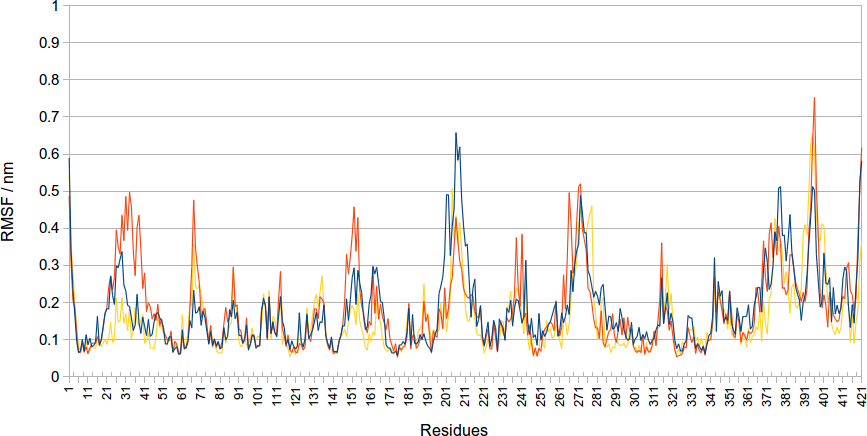
\includegraphics[width=0.8\textwidth,keepaspectratio=true]{graphics/acpMuphMonomerRmsf.png}}
		\caption[MupH atomic RMSF for the ACP-mupA3a:MupH monomer simulation.]{MupH atomic RMSF for the ACP-mupA3a:MupH monomer simulation. RMSF values for the residues in loop II (residue 198-214) can be seen larger than the residues on the loop I (residue 147-171). Blue, red and yellow lines represents the three replicates respectively.}
		\label{fig:acpMuphMonomerRmsf}
		\end{figure}					

		\setlength\fboxsep{5pt}
		\setlength\fboxrule{1.5pt}
		\begin{figure}[htbp]
		\centering
		\fbox{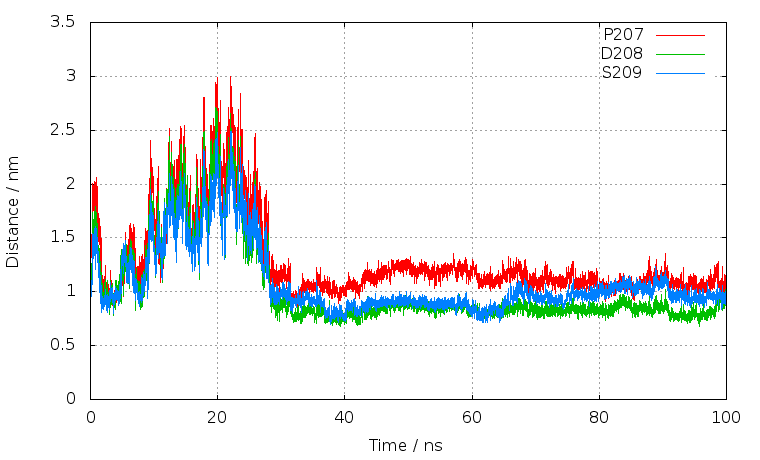
\includegraphics[width=0.8\textwidth,keepaspectratio=true]{graphics/AcpSpmMuphCyaSim0.png}}
		\caption[Distances between residues in loop I and loop II for the ACP-mupA3a:MupH monomer complex simulation replicate 1.]{Distances between residues in loop I and loop II for the ACP-mupA3a:MupH monomer complex simulation replicate 1. Distances were measured between the three C$ \alpha $ on the loop I (L150, M151 and I152) and three C$ \alpha $ on the loop II (P207, D208 and S209). Red, green and blue lines represents the average distance of P207, D208 and S209 respectively from the three residues on the loop I. The distance between the loops rise upto 3nm within 30 ns and then stabilized around 1nm.}
		\label{fig:AcpSpmMuphCyaSim0}
		\end{figure}	

		\setlength\fboxsep{5pt}
		\setlength\fboxrule{1.5pt}
		\begin{figure}[htbp]
		\centering
		\fbox{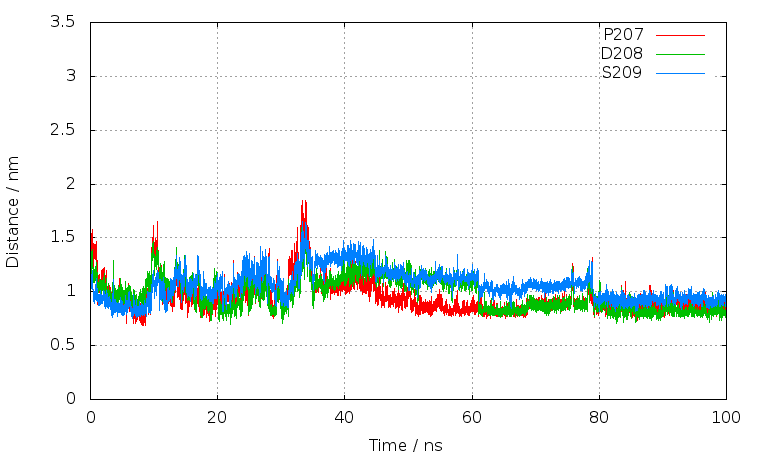
\includegraphics[width=0.8\textwidth,keepaspectratio=true]{graphics/AcpSpmMuphCyaSim1.png}}
		\caption[Distances between residues in loop I and loop II for the ACP-mupA3a:MupH monomer complex simulation replicate 2.]{Distances between residues in loop I and loop II for the ACP-mupA3a:MupH monomer complex simulation replicate 2. Distances were measured between the three C$ \alpha $ on the loop I (L150, M151 and I152) and three C$ \alpha $ on the loop II (P207, D208 and S209). Red, green and blue lines represents the average distance of P207, D208 and S209 respectively from the three residues on the loop I.}
		\label{fig:AcpSpmMuphCyaSim1}
		\end{figure}	

		\setlength\fboxsep{5pt}
		\setlength\fboxrule{1.5pt}
		\begin{figure}[htbp]
		\centering
		\fbox{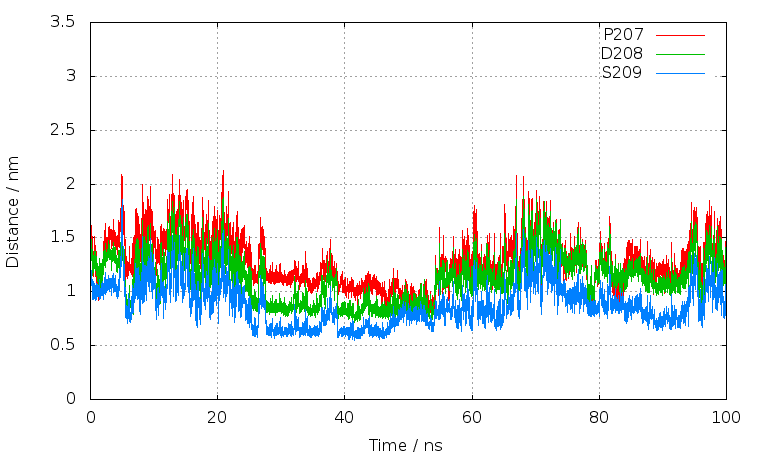
\includegraphics[width=0.8\textwidth,keepaspectratio=true]{graphics/AcpSpmMuphCyaSim2.png}}
		\caption[Distances between residues in loop I and loop II for the ACP-mupA3a:MupH monomer complex simulation replicate 3.]{Distances between residues in loop I and loop II for the ACP-mupA3a:MupH monomer complex simulation replicate 3. Distances were measured between the three C$ \alpha $ on the loop I (L150, M151 and I152) and three C$ \alpha $ on the loop II (P207, D208 and S209). Red, green and blue lines represents the average distance of P207, D208 and S209 respectively from the three residues on the loop I.}
		\label{fig:AcpSpmMuphCyaSim2}
		\end{figure}			

	\begin{table}[htbp]
	\caption{MupH simulation setup summary}
	\begin{tabularx}{\textwidth}{XXp{2cm}p{2cm}}
	\toprule[2pt]	
	\textbf{Structure} & \textbf{Ligand/modification} &\textbf{Simulation} & \textbf{Methods Section } \\
	\midrule[1pt]
	ACP-mupA3a:MupH monomer & MupH C115 acetylated \newline ACP-mupA3a cognate substrate  & 3 X 100 ns  &\ref{sec:mdAcpMuph}\\[5pt] 
	ACP-mupA3a:MupH dimer & MupH C115 acetylated \newline ACP-mupA3a cognate substrate  & 3 X 50 ns   & \ref{sec:mdAcpMuph}\\[5pt] 
	MupH monomer WT & -  & 3 X 50 ns & \ref{sec:muphCya}\\[5pt] 
	MupH acetylated C115 & C115 acetylated  & 3 X 50 ns & \ref{sec:muphCya}\\
	\bottomrule[2pt]
	\end{tabularx}
	\label{tab:mupHSimulationSetupSummary}
	\end{table}		

\newpage					
	A similar simulation with three independent replicates of 50 ns each, was also carried out with MupH in the dimeric form together with ACP-mupA3a docked to one of the monomers of MupH (as described in Section \ref{sec:mdAcpMuph}). It is quite likely that MupH exists as a dimer since other HMG-CoA orthologues exist as dimers and PIER analysis of a MupH model suggested an interface consistent with that seen in the crystal structure (Chapter 3, Section \ref{sec:RVandPIER}). The RMSF calculated for all atoms averaged per residue of MupH in the simulation of the ACP-mupA3a:MupH dimer complex showed lower values for the loop II than loop I (Figure \ref{fig:acpMuphDimerRmsf}). The distance measured between the two loops in the simulation of the ACP-mupA3a:MupH dimer complex also showed slightly lowered values for the largest distance reached between the two loops as compared to the ACP-mupA3a:MupH monomer simulation. The distance between the two loops remained constant throughout 50 ns in all the three replicates averaging around 1 nm and 1.5 nm with a rise up to 2 nm in two out of three replicates (Figures from \ref{fig:AcpSpmMuphCyaDimerSim0} to \ref{fig:AcpSpmMuphCyaDimerSim2}). Figure \ref{fig:AcpSpmMuphCyaDimerSim2} shows replicate 3 for the ACP-mupA3a:MupH dimer simulation in which the distance between the loops reached and remained at 2 nm and stayed plateaued for around 15 ns. These observations support the hypothesis that the dimer formation hinders the loop II movement, both in terms of its fluctuation on its position as well as its relative distance from loop I. This could be because loop II, being close to the dimer interface, interacts with the residues from the other monomer and hence stabilizes its position. Simulating the MupH dimer for a longer time scale might allow better sampling of the large ACP-mupA3a:MupH dimer complex which may not be enough within the 50 ns of simulations here. Due to lack of time it was not possible to run longer simulation on this complex. 

		\setlength\fboxsep{5pt}
		\setlength\fboxrule{1.5pt}
		\begin{figure}[htbp]
		\centering
		\fbox{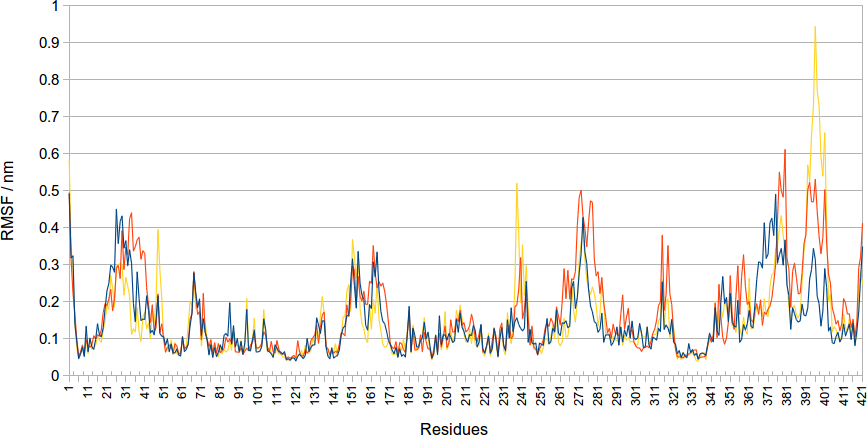
\includegraphics[width=0.8\textwidth,keepaspectratio=true]{graphics/acpMuphDimerRmsf.png}}
		\caption[ACP-mupA3a:MupH dimer complex, RMSF of all atoms averaged per residue of MupH.]{ACP-mupA3a:MupH dimer complex, RMSF of all atoms averaged per residue of MupH. RMSF values for the residues in loop II (residue 198-214) can be seen smaller than the residues on the loop I (residue 147-171). Blue, red and yellow lines represents the three replicates respectively.}
		\label{fig:acpMuphDimerRmsf}
		\end{figure}	

		\setlength\fboxsep{5pt}
		\setlength\fboxrule{1.5pt}
		\begin{figure}[htbp]
		\centering
		\fbox{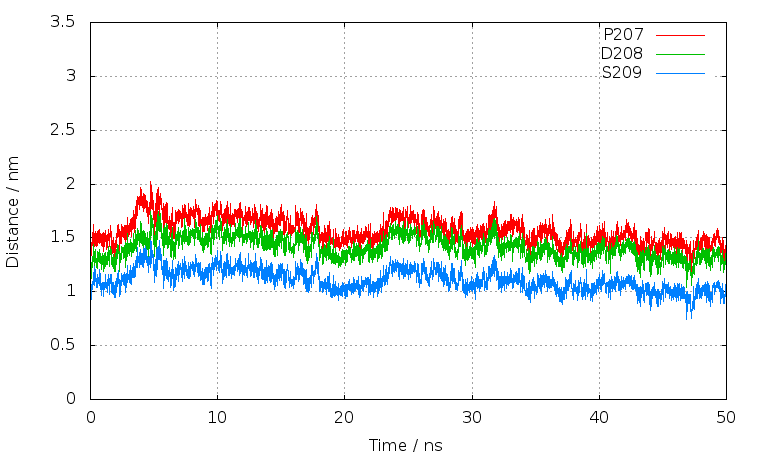
\includegraphics[width=0.8\textwidth,keepaspectratio=true]{graphics/AcpSpmMuphCyaDimerSim0.png}}
		\caption[ACP-mupA3a:MupH dimer complex simulation replicate 1, distance measured between the loop I and II over the time of 50ns.]{ACP-mupA3a:MupH dimer complex simulation replicate 1, distance measured between the loop I and II over the time of 50ns. Distances were measured between the three C$ \alpha $ on the loop I (L150, M151 and I152) and three C$ \alpha $ on the loop II (P207, D208 and S209). Red, green and blue lines represents the average distance of P207, D208 and S209 respectively from the three residues on the loop I.}
		\label{fig:AcpSpmMuphCyaDimerSim0}
		\end{figure}

		\setlength\fboxsep{5pt}
		\setlength\fboxrule{1.5pt}
		\begin{figure}[htbp]
		\centering
		\fbox{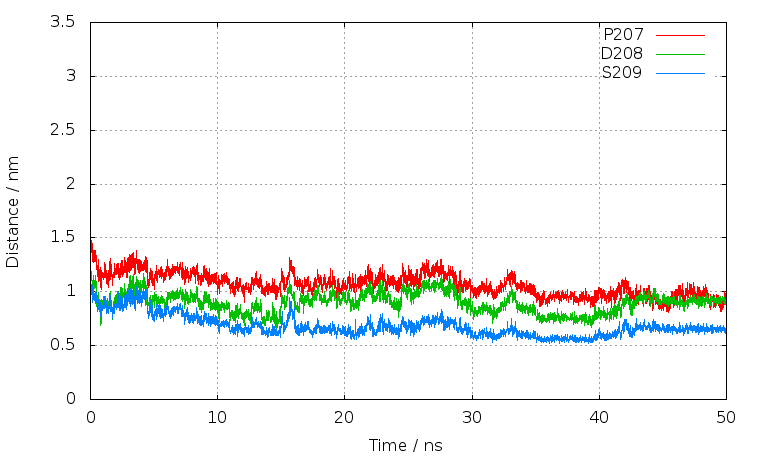
\includegraphics[width=0.8\textwidth,keepaspectratio=true]{graphics/AcpSpmMuphCyaDimerSim1.png}}
		\caption[ACP-mupA3a:MupH dimer complex simulation replicate 2, distance measured between the loop I and II over the time of 50ns.]{ACP-mupA3a:MupH dimer complex simulation replicate 2, distance measured between the loop I and II over the time of 50ns. Distances were measured between the three C$ \alpha $ on the loop I (L150, M151 and I152) and three C$ \alpha $ on the loop II (P207, D208 and S209). Red, green and blue lines represents the average distance of P207, D208 and S209 respectively from the three residues on the loop I.}
		\label{fig:AcpSpmMuphCyaDimerSim1}
		\end{figure}	

		\setlength\fboxsep{5pt}
		\setlength\fboxrule{1.5pt}
		\begin{figure}[htbp]
		\centering
		\fbox{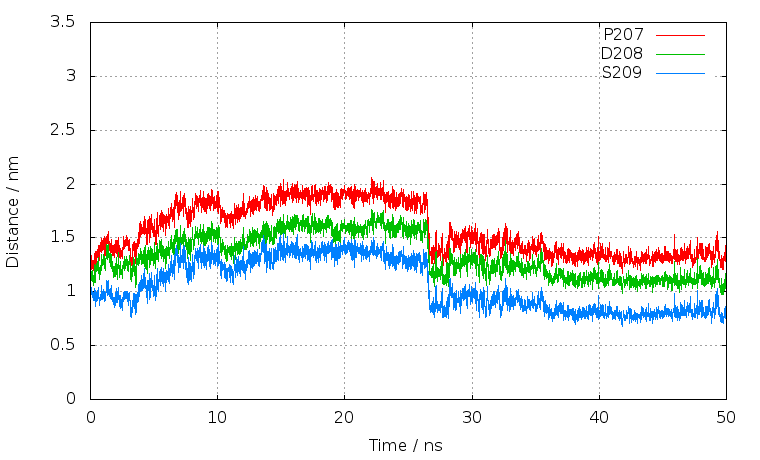
\includegraphics[width=0.8\textwidth,keepaspectratio=true]{graphics/AcpSpmMuphCyaDimerSim2.png}}
		\caption[ACP-mupA3a:MupH dimer complex simulation replicate 3, distance measured between the loop I and II over the time of 50ns.]{ACP-mupA3a:MupH dimer complex simulation replicate 3, distance measured between the loop I and II over the time of 50ns. Distances were measured between the three C$ \alpha $ on the loop I (L150, M151 and I152) and three C$ \alpha $ on the loop II (P207, D208 and S209). Red, green and blue lines represents the average distance of P207, D208 and S209 respectively from the three residues on the loop I.}
		\label{fig:AcpSpmMuphCyaDimerSim2}
		\end{figure}
\newpage
	One hypothesis that the loop movement may be triggered by the acetylation of the catalytic cysteine in MupH, that would signal MupH to open up the loops to let the ligand in. To test this hypothesis three independent 50 ns simulations were setup for the MupH monomer with C115 acetylated (as described in Section \ref{sec:muphCya}). RMSFs calculated for all atoms averaged per residue of MupH do not seem to be very different between loop I and II (Figure \ref{fig:muphCyaRmsf}). Figures \ref{fig:muphcyaSim0} to \ref{fig:muphcyaSim1} show the distances measured between the loops for the MupH monomer with C115 acetylated simulations. Distances measured in the three replicates remained below 2 nm averaging around 1 nm. These loop movements do not seem to be different from the movements seen in the ACP docked simulations. 

		\setlength\fboxsep{5pt}
		\setlength\fboxrule{1.5pt}
		\begin{figure}[htbp]
		\centering
		\fbox{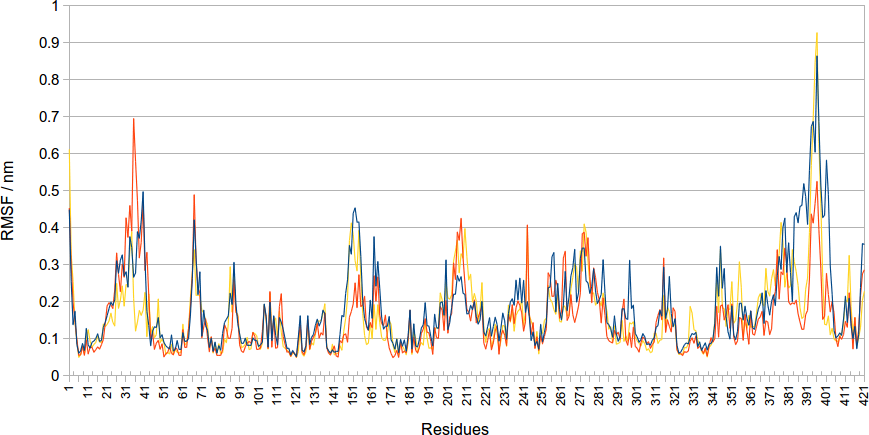
\includegraphics[width=0.8\textwidth,keepaspectratio=true]{graphics/muphCyaRmsf.png}}
		\caption[MupH monomer with C115 acetylated simulation, RMSF of all atoms averaged per residue of MupH.]{MupH monomer with C115 acetylated simulation, RMSF of all atoms averaged per residue of MupH. RMSF values for the residues in loop II (residue 198-214) and loop I (residue 147-171) does not seem to be very different from each other. Blue, red and yellow lines represents the three replicates respectively.}
		\label{fig:muphCyaRmsf}
		\end{figure}			
			
		\setlength\fboxsep{5pt}
		\setlength\fboxrule{1.5pt}
		\begin{figure}[htbp]
		\centering
		\fbox{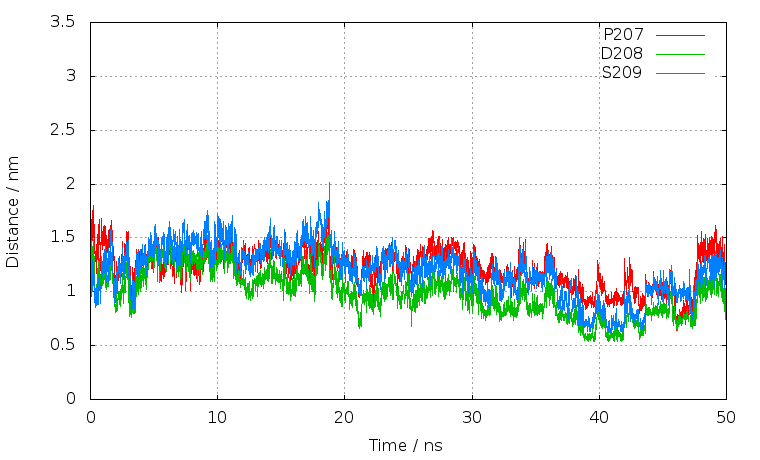
\includegraphics[width=0.8\textwidth,keepaspectratio=true]{graphics/muphcyaSim0.png}}
		\caption[MupH monomer with C115 acetylated simulation replicate 1, distance measured between the loop I and II over the time of 50ns.]{MupH monomer with C115 acetylated simulation replicate 1, distance measured between the loop I and II over the time of 50ns. CYA was the acytylated cysteine. Distances were measured between the three C$ \alpha $ on the loop I (L150, M151 and I152) and three C$ \alpha $ on the loop II (P207, D208 and S209). Red, green and blue lines represents the average distance of P207, D208 and S209 respectively from the three residues on the loop I.}
		\label{fig:muphcyaSim0}
		\end{figure}

		\setlength\fboxsep{5pt}
		\setlength\fboxrule{1.5pt}
		\begin{figure}[htbp]
		\centering
		\fbox{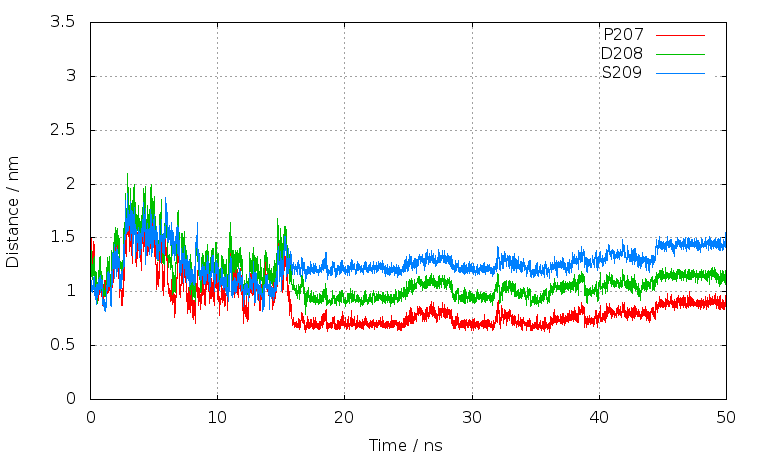
\includegraphics[width=0.8\textwidth,keepaspectratio=true]{graphics/muphcyaSim1.png}}
		\caption[MupH monomer with C115 acetylated simulation replicate 2, distance measured between the loop I and II over the time of 50ns.]{MupH monomer with C115 acetylated simulation replicate 2, distance measured between the loop I and II over the time of 50ns. CYA was the acytylated cysteine. Distances were measured between the three C$ \alpha $ on the loop I (L150, M151 and I152) and three C$ \alpha $ on the loop II (P207, D208 and S209). Red, green and blue lines represents the average distance of P207, D208 and S209 respectively from the three residues on the loop I.}
		\label{fig:muphcyaSim1}
		\end{figure}

		\setlength\fboxsep{5pt}
		\setlength\fboxrule{1.5pt}
		\begin{figure}[htbp]
		\centering
		\fbox{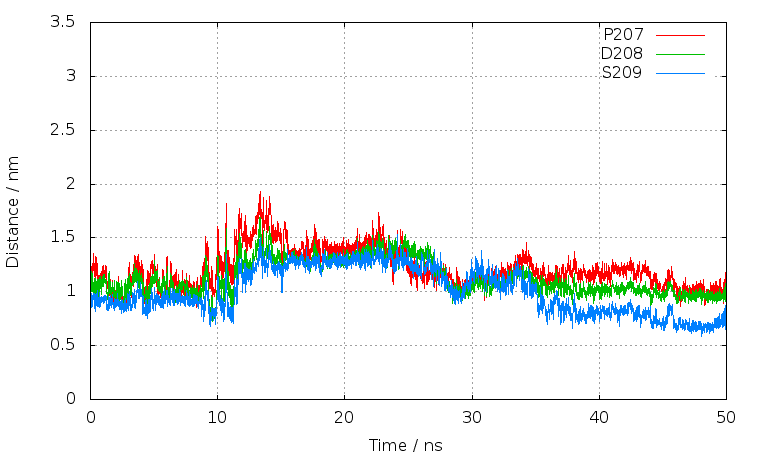
\includegraphics[width=0.8\textwidth,keepaspectratio=true]{graphics/muphcyaSim2.png}}
		\caption[MupH monomer with C115 acetylated simulation replicate 3, distance measured between the loop I and II over the time of 50ns.]{MupH monomer with C115 acetylated simulation replicate 3, distance measured between the loop I and II over the time of 50ns. CYA was the acytylated cysteine. Distances were measured between the three C$ \alpha $ on the loop I (L150, M151 and I152) and three C$ \alpha $ on the loop II (P207, D208 and S209). Red, green and blue lines represents the average distance of P207, D208 and S209 respectively from the three residues on the loop I.}
		\label{fig:muphcyaSim2}
		\end{figure}

\newpage
	The next obvious question was to see if this loop movement can be observed in the non-acetylated wild type MupH monomer, without being docked to ACP or with a ligand in its active site. If the loop movement is triggered by the docking of ACP or the presence of the ligand then there shouldn't be any huge fluctuation in the distances between the loops throughout the simulation. In order to test this hypothesis three independent simulations were run for a non-acetylated wild type MupH monomer for 50 ns each. RMSFs calculated for all atoms averaged per residue of MupH showed larger fluctuation in loop II than loop I, similar to the ACP-mupA3a:MupH monomer simulation (Figure \ref{fig:muphRmsf}). Figure \ref{fig:MuphSim1} shows the replicate 2 of the non-acetylated wild type MupH monomer simulation and it can be seen that the distance between the loops could fluctuate beyond 3 nm which was even more than with the bound ligand. Figures \ref{fig:MuphSim0} to \ref{fig:MuphSim2} show the distances measured for all the three replicates. These observations suggest that maybe this loop movement is intrinsic to MupH monomer proteins and it does not require binding of ACP or ligand to trigger it. However, it would also be interesting to see if this inter loop distance is consistent in the wild type ACP free MupH dimer as well. Due to lack of time it was not possible to run the non-acetylated wild type MupH dimer or MupH dimer with C115 acetylated simulations.		

		\setlength\fboxsep{5pt}
		\setlength\fboxrule{1.5pt}
		\begin{figure}[htbp]
		\centering
		\fbox{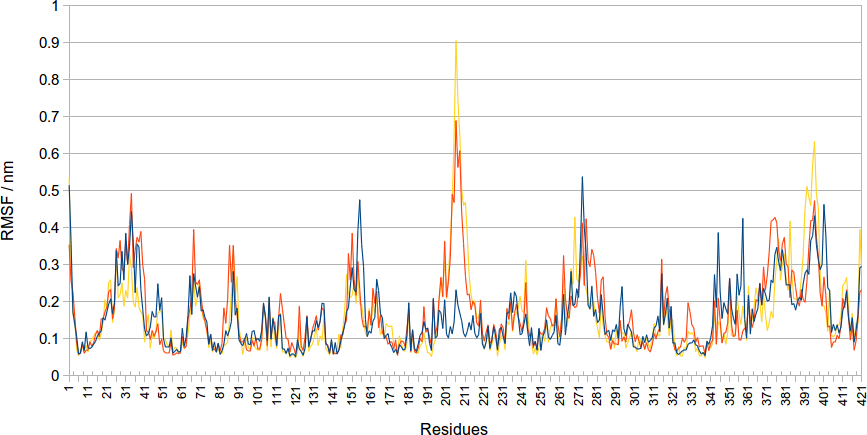
\includegraphics[width=0.8\textwidth,keepaspectratio=true]{graphics/muphRmsf.png}}
		\caption[Non-acetylated wild type MupH monomer simulation, RMSF of all atoms averaged per residue of MupH.]{Non-acetylated wild type MupH monomer simulation, RMSF of all atoms averaged per residue of MupH. RMSF values for the residues in loop II (residue 198-214) can be seen larger than the residues on the loop I (residue 147-171). Blue, red and yellow lines represents the three replicates respectively.}
		\label{fig:muphRmsf}
		\end{figure}	
		
		\setlength\fboxsep{5pt}
		\setlength\fboxrule{1.5pt}
		\begin{figure}[htbp]
		\centering
		\fbox{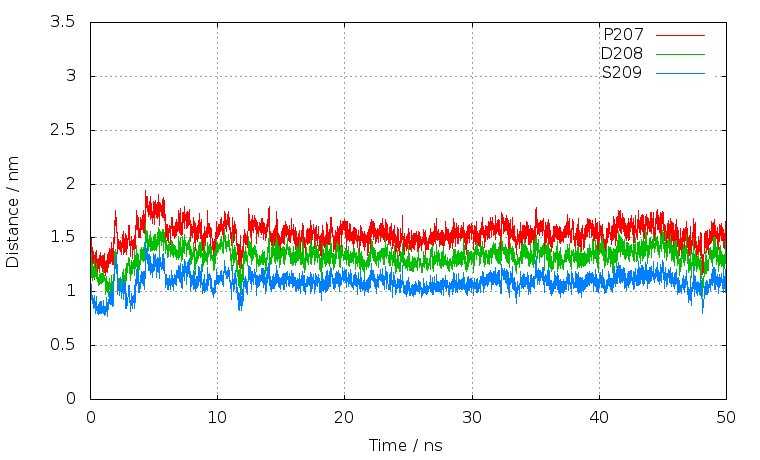
\includegraphics[width=0.8\textwidth,keepaspectratio=true]{graphics/MuphSim0.png}}
		\caption[Non-acetylated wild type MupH monomer simulation replicate 1, distance measured between the loop I and II over the time of 50ns.]{Non-acetylated wild type MupH monomer simulation replicate 1, distance measured between the loop I and II over the time of 50ns. Distances were measured between the three C$ \alpha $ on the loop I (L150, M151 and I152) and three C$ \alpha $ on the loop II (P207, D208 and S209). Red, green and blue lines represents the average distance of P207, D208 and S209 respectively from the three residues on the loop I.}
		\label{fig:MuphSim0}
		\end{figure}	

		\setlength\fboxsep{5pt}
		\setlength\fboxrule{1.5pt}
		\begin{figure}[htbp]
		\centering
		\fbox{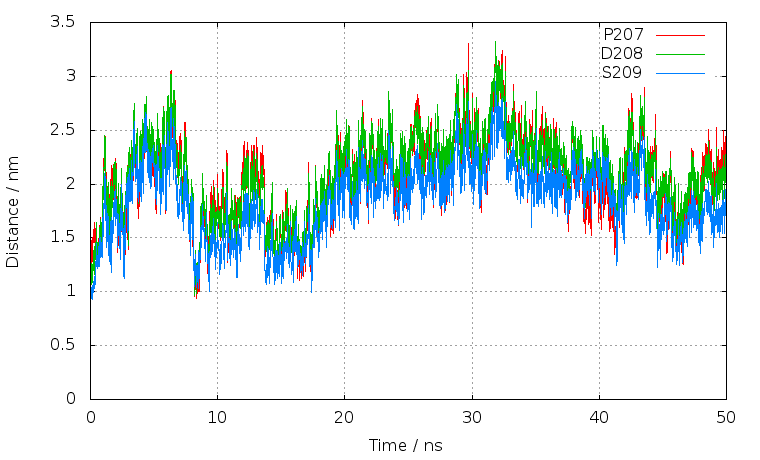
\includegraphics[width=0.8\textwidth,keepaspectratio=true]{graphics/MuphSim1.png}}
		\caption[Non-acetylated wild type MupH monomer simulation replicate 2, distance measured between the loop I and II over the time of 50ns.]{Non-acetylated wild type MupH monomer simulation replicate 2, distance measured between the loop I and II over the time of 50ns. Distances were measured between the three C$ \alpha $ on the loop I (L150, M151 and I152) and three C$ \alpha $ on the loop II (P207, D208 and S209). Red, green and blue lines represents the average distance of P207, D208 and S209 respectively from the three residues on the loop I.}
		\label{fig:MuphSim1}
		\end{figure}

		\setlength\fboxsep{5pt}
		\setlength\fboxrule{1.5pt}
		\begin{figure}[htbp]
		\centering
		\fbox{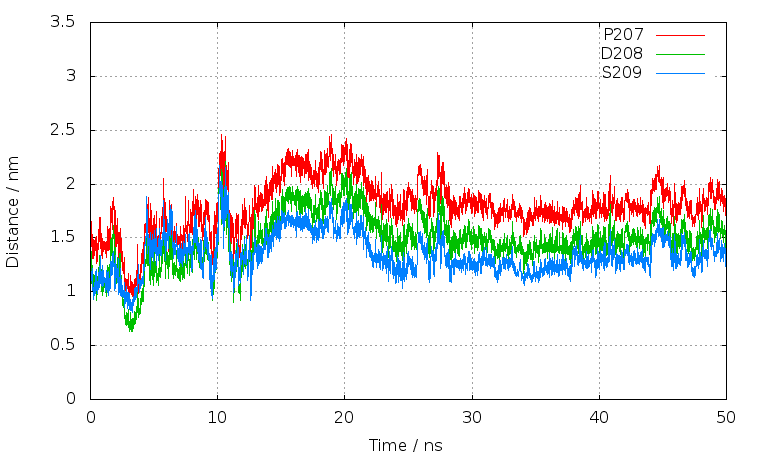
\includegraphics[width=0.8\textwidth,keepaspectratio=true]{graphics/MuphSim2.png}}
		\caption[Non-acetylated wild type MupH monomer simulation replicate 3, distance measured between the loop I and II over the time of 50ns.]{Non-acetylated wild type MupH monomer simulation replicate 3, distance measured between the loop I and II over the time of 50ns. Distances were measured between the three C$ \alpha $ on the loop I (L150, M151 and I152) and three C$ \alpha $ on the loop II (P207, D208 and S209). Red, green and blue lines represents the average distance of P207, D208 and S209 respectively from the three residues on the loop I.}
		\label{fig:MuphSim2}
		\end{figure}					
		

%
%		\setlength\fboxsep{5pt}
%		\setlength\fboxrule{1.5pt}
%		\begin{figure}[htbp]
%		\centering
%		\fbox{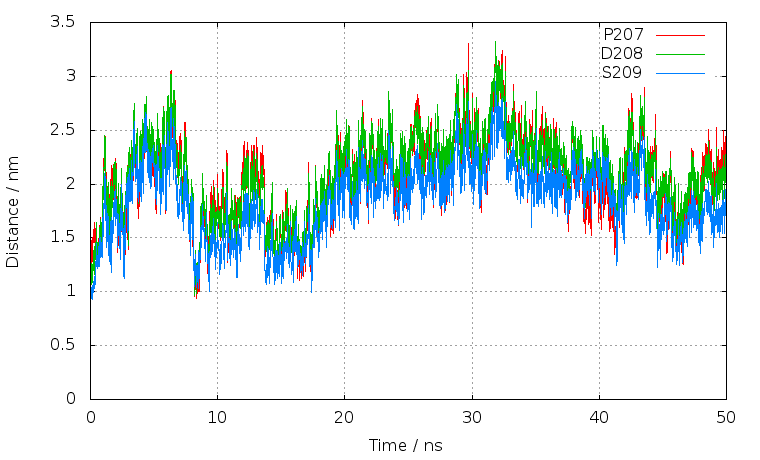
\includegraphics[width=\textwidth,keepaspectratio=true]{graphics/MuphSim1.png}}
%		\caption[Distance measured between the loop I and II over the time of 50ns in the MupH wild type replicate 2.]{Distance measured between the loop I and II over the time of 50ns in the MupH wild type replicate 2. CYA was the acytylated cysteine. Distances were measured between the three CA on the loop I (L150, M151 and I152) and three CA on the loop II (P208, D208 and S209). Red, green and blue lines represents the average distance of P207, D208 and S209 respectively from the three residues on the loop I.}
%		\label{fig:MuphSim1_iv}
%		\end{figure}				

\newpage		
\section{Discussion}
\label{sec:chap6Discussion}
	\subsection{A loop at the KS dimer interface appears to be responsible for the substrate specificity}
	\label{sec:chap6Discussionksspecificity}
	To find out what in the mup cluster is responsible for the addition of the 6-hydroxyl ($ \alpha $-hydroxyl), Dr. Joanne Hothersall from Prof. Thomas group carried out mutagenesis to delete \textit{mupA}, a tailoring gene. According to the position of occurrence of the 6-hydroxyl in the mupirocin (Figure \ref{fig:mupirocin}) it was hypothesized that MupA must be acting after MmpD. She found that the deletion strain produced mupiric acid but not mupirocin H \parencite{Wu2008}. It was inferred that this was formed by the release of an intermediate from module 4 of MmpD. Since no intermediates longer than mupiric acid were found this fits with the idea that MupA is acting after MmpD and if it is acting as a hydrolase, as hypothesised, then it suggests the non-hydroxylated monic acid intermediate cannot be recognised by the first extender domain of MmpA. Supposing that MupA was responsible for the addition of the 6-hydroxyl and that a lack of it would produce an intermediate without an $ \alpha $-hydroxyl, then what might be stopping KS-mupA2 from recognizing the non $ \alpha $-hydroxylated substrate? 
	
	Previous studies on the \textit{cis}-AT DEBS systems have shown that the KSs were able to be acylated by	unnatural substrates but were not able to carry out the elongation step, suggesting that the pathway stalled at the KS with the clogged intermediate \parencite{Watanabe2003}. In a recent study, \textcite{Busch2013} have shown a gate keeping mechanism in iterative  KSs from the \textit{cis}-AT aureothin system. However, studies conducted by \textcite{Menzella2005} showed PKSs accepting unnatural substrates in a \textit{cis}-AT system. Thus the substrate recognition mechanisms in the \textit{cis}-AT KSs are still not very well understood. 
	
	In the \textit{trans}-AT PKSs, \textcite{Nguyen2008} showed a strong correlation between the KS sequences and their preferred substrates. Based on this association of different substrates with different KS clades \textcite{Jenner2013} determined the basis of substrate specificity of a \textit{trans}-AT KS associated with accepting \bet-branched substrates. Using a novel mass spectrometry method they identified a position in the \textit{trans}-AT BaeL KS5 (bacillaene cluster) which is responsible for accepting only \bet-branched substrates. 
	
	To investigate the hypothesis that KS-mupA2 is specific for an $ \alpha $-hydroxylated precursor of monic acid the expected $ \alpha $-hydroxylate substrate was docked into a model of the KS-mupA2 dimer structure. A malonate molecule attached to the phosphopantetheine was also docked, while keeping the substrate C158 interaction, to mimic the decarboxylation stage of the Claisen condensation, with the phosphopantetheine attached to a modelled ACP-mupA2. The final docked conformation mimics the system ready to carry out the carbon-carbon bond formation and the acyl chain transfer to the phosphopantetheinylated ACP. Docking results revealed a motif, DNYK, within 5 \AA \ of the $ \alpha $-hydroxyl, in a loop contributed by the opposite subunit at the dimer interface. This loop connects an $ \alpha $-helix at its N-terminus to a \bet-strand at its C-terminus. The loop is similar to its counterpart in the thiomarinol TmpA module, whose synthetic pathway also produces a product hydroxylated at the same position, with TmpA and MmpA both having the conserved DNYK motif, but this loop is not conserved among the other KSs from the mupirocin and thiomarinol clusters. It was hypothesized that if this loop were to be swapped with the loops from KS-mupA1 or KS-mupA3 then the KS which does not process a substrate with an $ \alpha $-hydroxyl might allow the pathway to proceed further.
	
	There seems to be no similar DNYK motif present in the structures available in the PDB, determined by using the PDBe Motif webserver. Limiting the search to a motif in a helical context found only the Vaccinia Virus H7 protein (PDB ID 4W5X) containing this motif, however no ligand information was present. Looking into the structure of Vaccinia Virus H7 protein, the DNYK motif lies in a loop with the D of the motif (D56) at the C-terminus of a helix. Vaccinia Virus H7 protein has a unique fold with no sequence homology outside poxvirus family. The Vaccinia Virus H7 protein shares some similarity in secondary structure and surface properties with the PX domains,  which highlights surface residues K108, R109 and K112 forming a basic patch that are found to be important for binding phosphoinositides \parencite{Kolli2015}. However, the DNYK motif is structurally far away ($ \approx $25 \AA) from this basic patch and seems to have no role in the binding of phosphoinositides. Moreover, the loop points to solvent with no obvious interaction partners in the crystal lattice and in no way looks like a binding site. Limiting the search finding a DNYK motif in a loop context did not find any matching structure. Searching the motif without limiting the search for any secondary structure information found 31 structures with only a rabbit IGG fc fragment (PDB ID 2VUO) associated with ligand binding information. In the rabbit IGG fc fragment structure the backbone atoms of D389 are in van der Waals contact with an azide ion and the backbone nitrogen of N390 is making a hydrogen bond with the azide ion. The NZ of K392 is in van der Waals contact with the carbon of a formic acid molecule. Although this structure shows the DNYK motif to be in contact with the bound ligands, neither of the ligands carries an $ \alpha $-hydroxyl and the motif is on a $ \beta $-strand rather than on a loop or helix. Searching for DLYK, DLFK and DLLK variants did not yield any results different results from the DNYK motif search.
	
	To test the importance of this loop in recognizing the substrate, Miss. Y. Alsamrarraie from Prof. Thomas group inserted the key loop from KS-mupA1 into KS-mupA2 in a \textit{P. fluorescens} $ \Delta $\textit{mupA} strain and in the wild type \textit{P. fluorescens} NCIMB 10586. HPLC traces revealed a peak for both the mutant strains which was not detected in the parent \textit{P. fluorescens} $ \Delta $\textit{mupA} strain. This implies that the pathway has produced a full length substrate, and thus must have been successfully processed by the KS-mupA2 mutants. Thus, the chimera of KS-mupA2 with KS-mupA1 loop processed the substrates from WT and $ \Delta $mupA strains, presumed to be with and without $ \alpha $-hydroxyl. This could mean that the wild type KS-mupA2 serves as a checkpoint, which only allows an $ \alpha $-hydroxylated substrate to pass through and stalls the pathway in case of an $ \alpha $-dehydroxylated substrate. The structure of the metabolites produced are still to be confirmed from our collaborators at Bristol but is likely to be more hydrophobic than pseudomonic acid since it has a longer retention on the column, which is consistent with 6-dehydroxylated pseudomonic acid A. Once it is confirmed that the pathway has produced a molecule which lacks 6-hydroxyl further point mutations can be done to pin point the residue(s) responsible for the $ \alpha $-hydroxyl substrate specificity. Target point mutations may also help not only to modulate the specificity of KS-mupA2 towards accepting an non $ \alpha $-hydroxylated substrate but might also increase the amount of the metabolite produced as compared to swapping the whole loop. These insights would eventually lead towards successfully re-engineering \textit{trans}-AT KSs for accepting non natural substrates for the production of novel compounds, and may also apply to \textit{cis}-AT systems but further experiments are required. 
	 
	
	\subsection{Movement of MupH surface loops may have a role in ligand binding}
	\label{sec:chap6DiscussionLoopMovement}
	A large movement in two of the surface loops over the active site of MupH was seen in the simulations of an ACP-mupA3a:MupH complex (Chapter \ref{cha:chap4}, Section \ref{sec:chap4acpmuphmd}) with the ACP-mupA3a cognate substrate attached to the ACP and an acetyl molecule covalently bound to the catalytic C115 in MupH. This observation lead to the hypothesis that this large movement of MupH surface loops at the opening of the MupH active site might be assisting in accommodating the ligand inside the MupH active site. To test the hypothesis that the movement may be triggered either by the acetyl transfer to the catalytic C115 in MupH (see HMG-CoA reaction mechanism in Section \ref{fig:HMGCO-Areact}) or due the ACP-mupA3a docking to the MupH, three independent simulations were performed for each of the systems: ACP-mupA3a:MupH monomer, ACP-mupA3a:MupH dimer, MupH monomer with C115 acetylated and wild type MupH monomer structure.
	
	The simulations of the MupH monomer structure showed a general trend of larger movement in loop II, both in terms of its over all fluctuation (RMSF) and the distance between loop II and loop I, however, these fluctuations decreased in the simulations with a dimeric MupH. This could be because loop II, being close to the dimer interface, would interact with the residues from the other monomer, which might restrict its movement. It was also seen that the loops in the MupH monomer with ligand docked in the active site tend to have a large distance between them at the beginning of the simulation which decreases eventually and then remains at a roughly constant value of 10 \AA. One interpretation is that the MupH monomer structures may allow easy access to the active site until the substrate is bound. Whether these observations are biologically relevant or not is difficult to say with the available data. Multiple or longer simulation runs with monomeric and dimeric states might provide more evidence.
	
	Determining experimentally that MupH exists as a monomer or dimer may provide some insight into the simulations or may lead to further experiments.  In my previous analysis in Chapter \ref{cha:ACP-HCS}, Section \ref{sec:RVandPIER} real value evolutionary trace and PIER analysis showed a strong signal on the MupH surface corresponding to the dimer interface in the HMG-CoA homologue structure, hence suggesting that MupH is also a dimer. To test this experimentally a simple technique such as electrospray ionization mass spectrometry (ESI-MS) may be utilized. Since, ESI-MS is a \textquoteleft soft ionization\textquoteright technique which produces very few fragments, it would be straight forward to determine the mass of the whole MupH or MupH dimer (preserving the noncovlent interactions \parencite{Huang1993}). ESI-MS can also be utilized to quantify protein-protein association constant \parencite{BoeriErba2011}.